\documentclass[a4paper, 12pt]{report}

% ====================== PACKAGES ======================
\usepackage[english]{babel} % English and French language support
\usepackage[utf8]{inputenc} % UTF-8 encoding
\usepackage[T1]{fontenc} % Character encoding
\usepackage{amsmath, amssymb, amsfonts} % Math packages
\usepackage{amsthm} % Theorem package
\newtheorem{remark}{Remark}
\newtheorem{Proposition}{Proposition}
\newtheorem{theorem}{Theorem}
\newtheorem{definition}{Definition}
\newtheorem{assumption}{Assumption}
\newtheorem{example}{Example}
\newtheorem{lemma}{Lemma}
\usepackage{graphicx} % Required for inserting images
\usepackage{float} % Improved handling of floating elements
\usepackage{hyperref} % For hyperlinks
\usepackage{array, tabularx, multirow, multicol} % Table packages
\usepackage{caption, subcaption} % Caption and subcaption for figures and tables
\usepackage{setspace} % Set line spacing
\usepackage{abstract} % Abstract layout
\usepackage{color, xcolor} % Color handling
\usepackage{tcolorbox} % Colored boxes
\usepackage{lipsum} % For generating filler text
\usepackage{fancyhdr} % Fancy headers and footers
\usepackage{titlesec} % Section formatting
\usepackage{enumerate} % Enumerate with custom labels
\usepackage{booktabs, colortbl} % Improved table formatting
\usepackage{geometry} % To define page margins
\usepackage{longtable} % For tables spanning multiple pages
\usepackage{listings}
\usepackage{bm}

% ====================== COMMANDS ======================
\providecommand{\abs}[1]{\lvert#1\rvert} % Absolute value command
\DeclareMathOperator{\sign}{sign} % Sign function

% ====================== PAGE GEOMETRY ======================
\geometry{top=2cm, bottom=3cm, left=2cm, right=2cm} % Adjust top margin to provide space for header
\setlength{\headheight}{45pt} % Increase headheight to fit header content
\setlength{\headsep}{20pt} % Add space between header and text

% ====================== PDF METADATA ======================
\hypersetup{ % Information about the PDF document
    pdfauthor = {Premier Auteur}, % Authors
    pdftitle = {Nom du Projet - Sujet du Projet}, % Title
    pdfsubject = {Mémoire de Projet}, % Subject
    pdfkeywords = {Tag1, Tag2, Tag3}, % Keywords
    pdfstartview={FitH}, % Adjust page width to screen width
    colorlinks=true, % Colored links
    citecolor=black, % Citation links color
    filecolor=black, % File links color
    linkcolor=black, % Internal links color
    urlcolor=black % URL links color
}

\lstset{
    language=Python,
    basicstyle=\ttfamily\footnotesize,
    keywordstyle=\color{blue},
    commentstyle=\color{orange},
    stringstyle=\color{red},
    showstringspaces=false,
    numberstyle=\tiny\color{gray},
    numbers=left,
    stepnumber=1,
    numbersep=5pt,
    frame=single,
    breaklines=true,
    backgroundcolor=\color{lightgray},
    captionpos=b,
    tabsize=4,
    morekeywords={Material, self},
}

% Définir les couleurs pour le code MATLAB
\definecolor{codegreen}{rgb}{0,0.6,0}
\definecolor{codegray}{rgb}{0.5,0.5,0.5}
\definecolor{codepurple}{rgb}{0.58,0,0.82}
\definecolor{backcolour}{rgb}{0.95,0.95,0.92}

% Définir le style pour MATLAB
\lstdefinestyle{mystyle}{
    backgroundcolor=\color{backcolour},
    commentstyle=\color{codegreen},
    keywordstyle=\color{magenta},
    numberstyle=\tiny\color{codegray},
    stringstyle=\color{codepurple},
    basicstyle=\ttfamily\footnotesize,
    breakatwhitespace=false,
    breaklines=true,
    captionpos=b,
    keepspaces=true,
    numbers=left,
    numbersep=5pt,
    showspaces=false,
    showstringspaces=false,
    showtabs=false,
    tabsize=2
}

% Définir l'environnement MATLAB
\lstnewenvironment{MATLAB}[1][]
{
    \lstset{
        style=mystyle,
        language=Matlab,
        #1
    }
}{} % End of MATLAB environment

% ====================== HEADER AND FOOTER ======================
\pagestyle{fancy} % Enable fancy headers and footers
\fancyhf{} % Clear all header and footer fields

\fancyhead[L]{ % Left header
    \begin{minipage}{1.5cm}
        \centering
        
\includegraphics[width=0.80\textwidth]{imgs/LogoCN_Q.pdf}
    \end{minipage}
    \begin{minipage}{12cm}
        \small \textsc{École}\\
        \small \textsc{Centrale}\\
        \small \textsc{de Nantes}\\
    \end{minipage}
}
\fancyhead[R]{ % Right header
    \begin{minipage}{4.8cm}
        \raggedleft
    \end{minipage}
    \begin{minipage}{1.5cm}
        \centering
        
\includegraphics[width=2\textwidth]{imgs/TU_Ilmenau_Logo_black_green.svg.png}
    \end{minipage}
}
\fancyfoot[R]{\large \textbf{\thepage}} % Right footer with page number

\renewcommand{\headrulewidth}{0.2pt} % Header rule width
\renewcommand{\footrulewidth}{0.2pt} % Footer rule width

% ====================== SECTION FORMATTING ======================
\titleformat{\chapter}[display]
    {\normalfont\bfseries}{}{0pt}{\Large}
\titlespacing*{\chapter}{0pt}{-20pt}{20pt}

% ====================== BEGIN DOCUMENT ======================
\begin{document}
\pagenumbering{arabic} % Start page numbering in arabic numerals
\renewcommand{\labelenumii}{\arabic{enumi}.\arabic{enumii}}

% Title page
\begin{titlepage}
    \centering
    \vspace*{0cm}
    
\includegraphics[width=0.3\textwidth]{imgs/LogoCN_Q.pdf}\hfill
    
\includegraphics[width=0.3\textwidth]{imgs/TU_Ilmenau_Logo_black_green.svg.png}
    
    \vspace{3cm}
    
    \Huge\textbf{Engineering Internship Report}\\
    \vspace{1cm}
    \LARGE\textbf{Breaking Algebraic Loops}\\
    \LARGE\textbf{in Sliding Mode Control}
    
    \vfill
    
    \Large\textbf{Author:} Matis Viozelange\\[0.3cm]
    \Large\textbf{Supervisor:} Niclas Tietze\\
    
    \vfill
    
    \Large\textbf{Technische Universität Ilmenau}\\
    \vspace{0.5cm}
    \Large\textbf{École Centrale Nantes}
    
    \vspace{1.5cm}
    
    \Large\textbf{Internship Period:}\\
    \Large 31/03/2024 -- 21/09/2024

    \vspace*{1cm}
\end{titlepage}

% Blank page
\newpage
\thispagestyle{empty}
~

% Abstract section
\begin{abstract}
    The project aimed to address the challenges posed by algebraic 
    loops in sliding mode control algorithms. These loops occur when 
    state-dependent perturbations interact with the control signal, 
    creating circular dependencies that complicate system stability 
    and performance. The research explored dynamic methods and international 
    collaborations to simplify convergence proofs without redesigning the 
    entire controller. This work is crucial for enhancing the robustness 
    and efficiency of control systems in various industrial applications.
    The other topic of the report is the peaking phenomenon in Model Following
    Control (MFC) and its implementation on a Matlab simulation and a real
    system.
\end{abstract}




% Table of contents
\tableofcontents
\thispagestyle{empty}
% \setcounter{page}{0}

\listoffigures

% Espacement entre les lignes d'un tableau
\renewcommand{\arraystretch}{1.5}

%====================== INCLUSION DES PARTIES ======================

~
\thispagestyle{empty}
%recommencer la numérotation des pages à "1"
%\setcounter{page}{0}
\newpage

\input{Sections/présentation_team_et_cadre-scientifique}
\chapter{Introduction}

This report documents my international mobility experience as part of my 
TFE at Centrale Nantes. The internship was conducted at Technische 
Universität Ilmenau, located in the heart of Thuringia, Germany and led 
by my supervisor PhD. student Niclas Tietze. 
Known for its rigorous academic environment and focus on applied sciences, 
TU Ilmenau provided an ideal setting for my research project.

The Institut für Automatisierungs und Systemtechnik at Technische 
Universität Ilmenau is a dynamic research group specializing in 
advanced control systems and automation technologies. Led by Prof. 
Johann Reger, the team comprises 14 members, including professors, 
researchers, and PhD students, all contributing to various projects in 
the field of control engineering. The primary objective of my internship 
was to work on the project titled Resolution of algebraic loops 
in sliding mode control approaches. This project aimed to address the 
challenges posed by algebraic loops in sliding mode control algorithms, 
particularly focusing on state-dependent disturbances that create circular 
dependencies with the control signal which complicate the already known
stability proofs for controller of the super-twisting type.

During my internship, I also had the opportunity to study and implement 
the Model Following Control (MFC) strategy, which is a robust control 
technique designed to ensure that a system's output follows a desired 
reference model, even in the presence of uncertainties and disturbances. 
MFC is particularly useful in applications requiring precise tracking of 
a reference trajectory, such as in robotics, aerospace, and automotive 
systems. One of the key challenges addressed by MFC is the peaking 
phenomenon, which occurs in high gain control systems and can lead to 
large, temporary deviations in the system's response. The MFC strategy 
mitigates this phenomenon by using a two-loop structure: the Model Control 
Loop (MCL) for nominal control and the Process Control Loop (PCL) for 
perturbation compensation.

Throughout this report will be provided a first part on the MFC strategy, the 
theoretical background then a focus on its assets in both implementation and 
performance compared to high gain control which is very close to MFC.
Next will be a second part on the algebraic loops resolution in sliding mode
control approaches, with the context of the problem, the state of the art
and the methodology used to solve this problem. A method will be proposed 
for a certain class of perturbation and then clues and ideas for the
general case will be given.

This internship has not only enhanced my technical knowledge in control 
systems but also provided me with a deeper understanding of German culture 
and academic practices. I am grateful for the opportunity to have been a 
part of such a dynamic and innovative research team.


\chapter{Model Following Control Theory and Peakin Phenomenon}

% =============================== Introduction =============================== %
%                                                                              %
%                                                                              %
%                                                                              %
% ============================================================================ %

\section{Introduction}

\subsection{Context and Motivation}

The model following control (MFC) strategy is a robust control technique that aims to ensure that 
a system's output follows a desired reference model, even in the presence of uncertainties and disturbances. 
This approach is particularly useful in applications where precise tracking of a reference trajectory 
is essential, such as in robotics, aerospace, and automotive systems. 

It based on the idea to keep or stay as close as possible to a High Gain control. The issue with this 
kind of controller being the high input values that can occure when the system state is far away 
from the desired setpoint or trajectory. The question is, how can one prevent such behavior while still achieving good performance and maintaining a simple control law to implement on a real system?

The idea at the begining is to divide the process into two loops, one to keep track of the model and its behavior 
regarding the desired trajectory and one very quick to correct the error between the model and the real system 
due to initial conditions or perturbations.

The goals of this Chapter's work can be enumerated as follows:

\begin{enumerate}
    \item Present the Model Following Control (MFC) strategy, including its theoretical 
    foundations and implementation details.
    \item Implement this theory on a Matlab Crane simulation.
    \item Implement this theory on a real 3D crane system.
    \item Analyze the performances and highlight the peaking phenomenon attenuation.
\end{enumerate}

\subsection{Crane Presentation}

As said before, the MFC strategy will be implemented on a crane system. The crane is a common 
industrial machine used for lifting and moving heavy loads. It consists of a trolley that moves along a 
horizontal beam, with a hoist mechanism that raises and lowers the load. The primary objective 
of controlling a crane system is to ensure precise positioning of the load while minimizing 
oscillations and ensuring safety.

\begin{figure}[htbp]
    \centering
    \rotatebox{270}{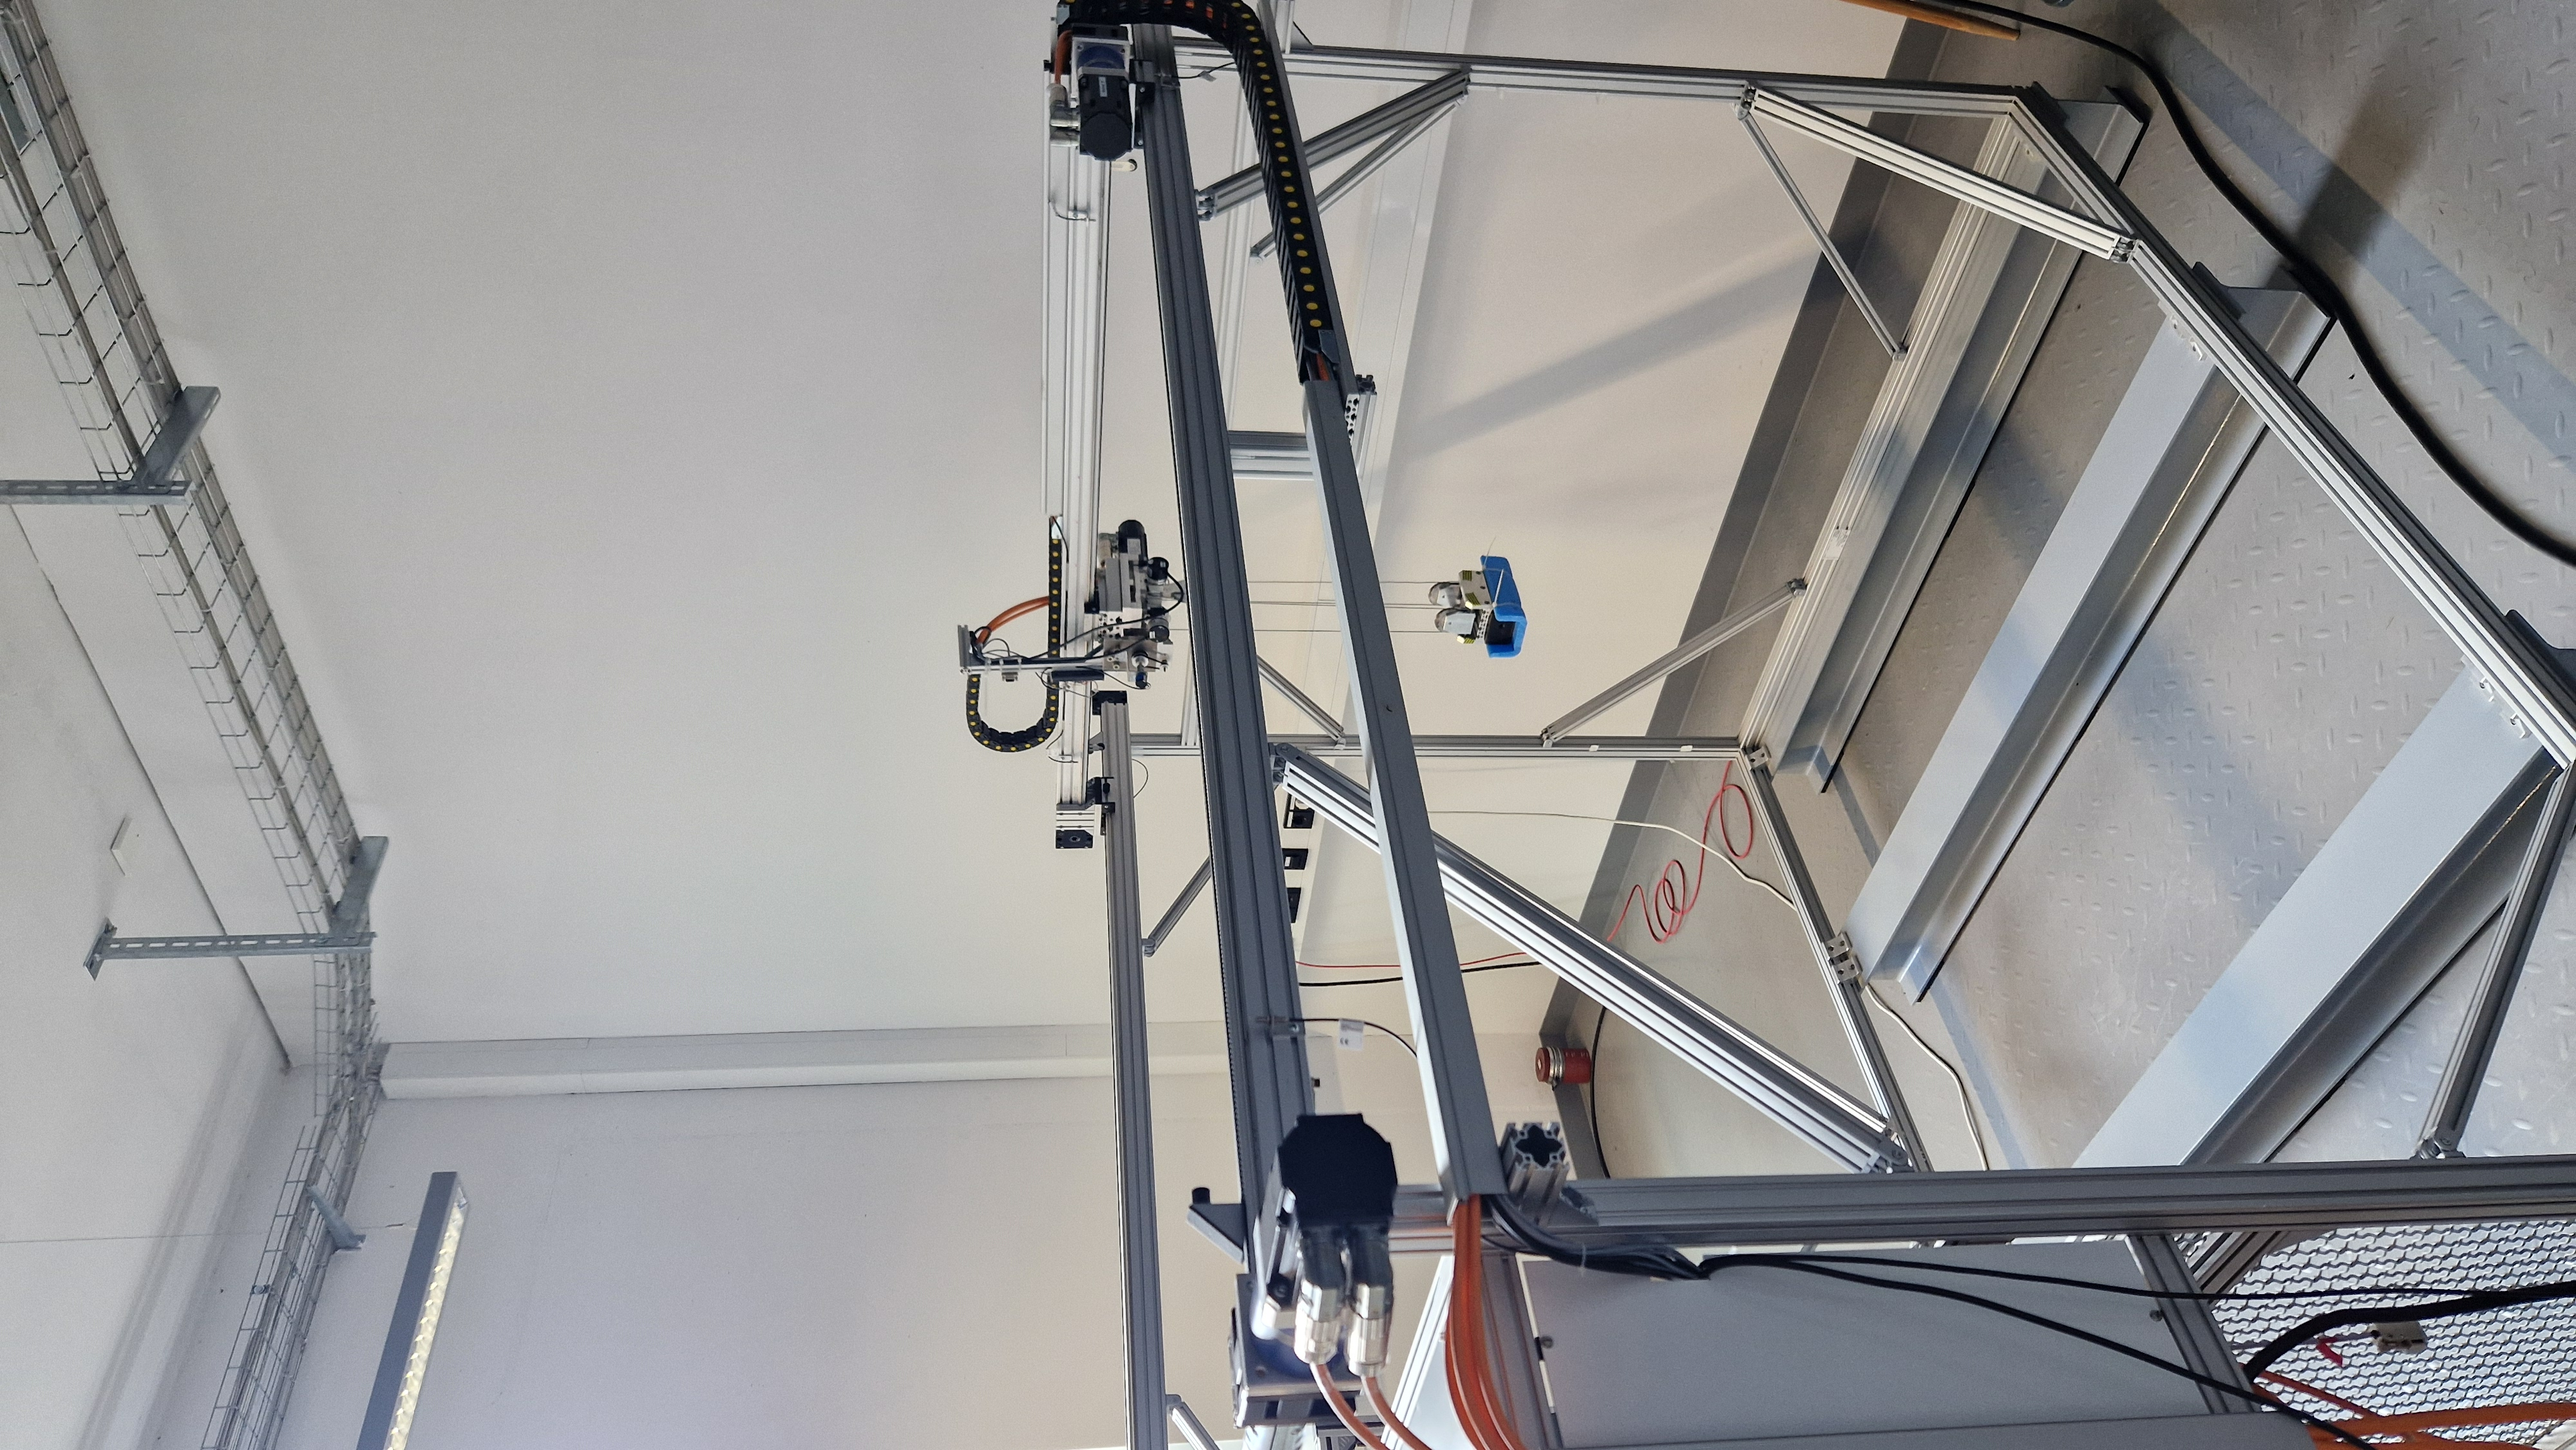
\includegraphics[width=0.5\linewidth]{imgs/section1/General.jpg}}
    \caption{Real 3-dimensional overhead crane.}
    \label{fig:Real_3D_Crane}
\end{figure}

The Figure~\ref{fig:Real_3D_Crane} shows the real crane system on which the MFC strategy will be tested. 
We will see in the following sections how to model this system and apply the MFC strategy to achieve 
good performance while mitigating the peaking phenomenon.

First of all, let's present the MFC strategy and its theoretical background. Then, we will 
describe the crane model and its dynamics in detail.

\newpage

% =============================== Model Following Control ========================= %
%                                                                                   %
%                                                                                   %
%                                                                                   %
% ================================================================================= %
\section{Model Following Control}
\label{sec:model-following-control}


\subsection{Overview}

The Model Following Control (MFC) Loop, described in Figure~\ref{fig:MFC_Control_Loop}, 
consists of two primary loops: the Model Control Loop (MCL) and the Process Control Loop (PCL). 
The MCL is used for nominal control based on a theoretical model of the plant. It provides a nominal 
output \(y^*\), nominal states \(x^*\), and a nominal control input \(u^*\). The PCL then uses these nominal 
states as a reference to compensate for perturbations with the control input \(\tilde{u}\). The composite 
control input is the sum of \(\tilde{u}\) and \(u^*\), acting as a feedforward. The MCL assumes no 
uncertainties, allowing the model controller to be tuned to achieve optimal tracking of the desired 
output \(y_d\).

The theoretical foundation for this controller architecture is drawn from the work in \cite{Willkomm2023MFC}.

\begin{figure}[htbp]
    \centering
    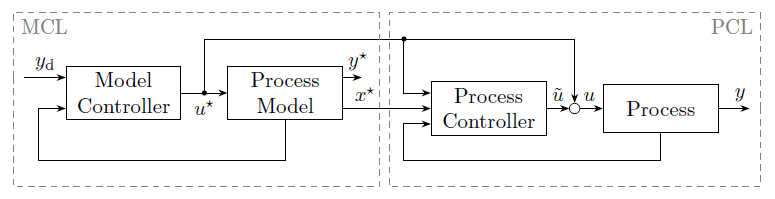
\includegraphics[width=0.8\textwidth]{imgs/section1/MFC_scheme.PNG}
    \caption{Model Following Control block diagram with model control loop process and control loop \cite{Willkomm2023MFC}.}
    \label{fig:MFC_Control_Loop}
\end{figure}

\subsection{General Equation}

Consider the flat system:

\begin{equation}
    \label{eq:flat_sys_reduced1}
    \left\{
        \begin{aligned}
            \dot{\boldsymbol{\xi}} &= A\boldsymbol{\xi} + B\big(a(\boldsymbol{\xi}) + b(\boldsymbol{\xi})u + \Delta(\boldsymbol{\xi}, t) \big) \\
            y &= C\boldsymbol{\xi}
        \end{aligned}
    \right.
\end{equation}

where \(\boldsymbol{\xi}(t) \in \mathbb{D}_\xi \subseteq \mathbb{R}^n\) denotes the states, 
\(\Delta: \mathbb{D}_{\xi} \times \mathbb{R}^+ \rightarrow \mathbb{R}\) are the unknown 
perturbations, \(y(t) \in \mathbb{R}\) is the output, and \(u(t) \in \mathbb{R}\) is the input. TThe relative degree is \(n \ge 1\).


\begin{remark}
This analysis considers a SISO system. However, we will see later that the crane system is a MIMO system.
We can address this issue by decoupling the system into several SISO systems with the exact feedback linearization
which will be explained later.
\end{remark}

The matrices \(A\), \(B\), and \(C\) are defined as:
\begin{align}
    A &=
    \begin{bmatrix}
    0 & 1 & 0 & \cdots & 0 \\
    0 & 0 & 1 & \cdots & 0 \\
    \vdots & \vdots & \ddots & \ddots & \vdots \\
    0 & 0 & \cdots & 0 & 1 \\
    0 & 0 & \cdots & 0 & 0
    \end{bmatrix}
    \in \mathbb{R}^{n \times n}, \quad
    B =
    \begin{bmatrix}
    0 \\
    0 \\
    \vdots \\
    0 \\
    1
    \end{bmatrix}
    \in \mathbb{R}^n, \\
    C &=
    \begin{bmatrix}
    1 & 0 & \cdots & 0
    \end{bmatrix}
    \in \mathbb{R}^{1 \times n}.
\end{align}

With no surprise as the SISO system is considered to be flat. The perturbation \(\Delta(\xi, t)\) is assumed 
to be bounded and Lipschitz continuous with respect to the states \(\xi\). And, we don't take the case of a system
with zero dynamics but it doesn't change a lot the analysis as in \cite{Willkomm2023MFC} they are considered
to be input to state stable and the exact linearization of the crane system will be a flat system.

Let's divide the control into a nominal part \(u^*\) that stabilizes a flat system with no perturbations
and a perturbation compensating part \(\tilde{u}\) by writing the eq~\ref{eq:flat_sys_reduced1} differently.

\subsection{Model Control Loop (MCL)}

An analysis of the control loop dynamics is conducted in two stages. First, the Model Control 
Loop (MCL) is considered, which replicates system \eqref{eq:flat_sys_reduced1} without perturbations \(\Delta\):

\begin{equation}
    \label{eq:MCL_open_loop}
    \dot{\boldsymbol{\xi}^*} = A\boldsymbol{\xi}^* + B\big(a(\boldsymbol{\xi}^*) + b(\boldsymbol{\xi}^*)u^* \big).
\end{equation}

The input is decomposed as \(u = \tilde{u} + u^*\), where \(u^*\) is the output of the MCL and 
\(\tilde{u}\) is the output of the PCL (process control loop). We define the error states as 
\(\tilde{\boldsymbol{\xi}} = \boldsymbol{\xi} - \boldsymbol{\xi}^*\) as the difference between the actual and model states, and the open-loop 
dynamics of the MFC are:

\begin{align}
    \dot{\boldsymbol{\xi}}^* &= A\boldsymbol{\xi}^* + B \left( a(\boldsymbol{\xi}^*) + b(\boldsymbol{\xi}^*) u^* \right), \\
    \dot{\tilde{\boldsymbol{\xi}}} &= A\tilde{\boldsymbol{\xi}} + B \left( \tilde{a}(\boldsymbol{\xi}^*, \tilde{\boldsymbol{\xi}}, u^*) + b(\boldsymbol{\xi}^* + \tilde{\boldsymbol{\xi}}) \tilde{u} + \Delta(\boldsymbol{\xi}^* + \tilde{\boldsymbol{\xi}}, t)  \right),
\end{align}

where :

\begin{align}
    \tilde{a}(\boldsymbol{\xi}^*, \tilde{\boldsymbol{\xi}}, u^*) &= a(\boldsymbol{\xi}^* + \tilde{\boldsymbol{\xi}}) - a(\boldsymbol{\xi}^*) + \left( b(\boldsymbol{\xi}^* + \tilde{\boldsymbol{\xi}}) - b(\boldsymbol{\xi}^*) \right) u^*.
\end{align}

To ensure closed-loop stability, a feedback linearization law is applied to the MCL:

\begin{equation}
    \label{eq:MCL_control_law}
    u^* = -\frac{a(\boldsymbol{\xi}^*) + v^*}{b(\boldsymbol{\xi}^*)}.
\end{equation}

The design of \(v^*\) is based on the error dynamics within the MCL: \(\tilde{\boldsymbol{\xi}}^* = \boldsymbol{\xi}^* - \boldsymbol{\xi}_d\), 
representing the deviation between the model and desired states. The associated error dynamics are:

\begin{align}
    \dot{\tilde{\boldsymbol{\xi}}}^* &= A\tilde{\boldsymbol{\xi}}^* + B(v^* - y_d^{(r)}).
\end{align}

The new input \(v^*\) is chosen as:
\begin{equation}
    v^* = y_d^{(r)} + K\tilde{\boldsymbol{\xi}}^*,
\end{equation}

where \(K = [-\alpha_0, -\alpha_1, \ldots, -\alpha_{r-1}] \in \mathbb{R}^{1 \times n}\) is selected 
such that the matrix \(A + BK\) is Hurwitz. The closed-loop dynamics of the MCL become:

\begin{align}
    \dot{\tilde{\boldsymbol{\xi}}}^* &= (A + BK)\tilde{\boldsymbol{\xi}}^*.
\end{align}

And stabilizes the MCL dynamics. Now we can focus on the perturbation compensation with the process control loop
which will be addressed with the same idea as the MCL.

\subsection{Process Control Loop (PCL)}
The process control loop is designed to counter perturbations and model uncertainties using a high-control 
gain approach. This approach allows for rapid error correction and improved robustness without high input 
work on the model/desired states error. The desired output trajectory \(y_d(t) \in \mathbb{R}\) is assumed 
to be at least \(n\)-times continuously differentiable. The desired external 
states \(\boldsymbol{\xi}_d(t) \in \mathbb{D}_{\boldsymbol{\xi}_d} \subseteq \mathbb{R}^n\) are generated by:


\begin{equation}
    \dot{\boldsymbol{\xi}}_d = A\boldsymbol{\xi}_d + B\boldsymbol{y}_d^{(n)}.
\end{equation}
The error states of the PCL are defined as \(\tilde{\boldsymbol{\xi}} = \boldsymbol{\xi} - \boldsymbol{\xi}^*\). The open-loop error dynamics are:

\begin{align}
    \dot{\tilde{\boldsymbol{\xi}}} &= A\tilde{\boldsymbol{\xi}} + B\left(\tilde{a}(\boldsymbol{\xi}^*, \tilde{\boldsymbol{\xi}}, u^*) + b(\tilde{\boldsymbol{\xi}}^* + \tilde{\boldsymbol{\xi}}) \tilde{u} + \Delta(\tilde{\boldsymbol{\xi}}^* + \tilde{\boldsymbol{\xi}}, t) \right).
\end{align}

The process controller is designed using a feedback linearizing control law on the same principle as the MCL:

\begin{equation}
    \tilde{u} = \frac{-\tilde{a}(\boldsymbol{\xi}^*, \tilde{\boldsymbol{\xi}}, u^*) + \tilde{K}\tilde{\boldsymbol{\xi}}}{b(\boldsymbol{\xi}^* + \tilde{\boldsymbol{\xi}})},
\end{equation}

where \(\tilde{K} = KD^{-1}\varepsilon^{-1}\) with \(D = \text{diag}(\varepsilon^{n}, \varepsilon^{n-1}, 
\ldots, 1)\) and \(0 < \varepsilon < 1\) is a time scaling parameter.

A time scaling change of variable is introduced into the PCL to make the time scaling factor \(\varepsilon\)
of the high-gain control appears in the closed loop dynamics to make its action on the perturbation compensation
appears and allow us to find a mathematical condition on \(\varepsilon\) to counter the perturbations.

\begin{equation}
    \zeta = D^{-1}\tilde{\boldsymbol{\xi}}.
\end{equation}

The closed-loop overall dynamics of the MFC scheme for set-point and trajectory tracking are:

\begin{align}
    \label{eq:closed_loop_overall_dynamics}
    \dot{\tilde{\boldsymbol{\xi}}}^* &= (A + BK)\tilde{\boldsymbol{\xi}}^*, \\
    \varepsilon\dot{\zeta} &= (A + BK)\zeta + \varepsilon B \left(\Delta(\boldsymbol{\xi}_d + \tilde{\boldsymbol{\xi}}^* + D(\zeta, t)) \right).
\end{align}

Here in \ref{eq:closed_loop_overall_dynamics}, the time scaling factor \(\varepsilon\) appears in the
closed-loop dynamics only on the second equation part where \(\Delta\) appears, allowing us to find a
mathematical condition on \(\varepsilon\) to counter the perturbations as it was said before.

The key points of this control strategy are:

    \begin{itemize}
    \item If \( A + BK \) is Hurwitz, the eigenvalues of the error dynamics (without time-scaling) can 
    be shifted arbitrarily far to the left of the imaginary axis as \( \epsilon \rightarrow 0 \).
    \item Theoretically, the error dynamics can be made to converge arbitrarily quickly.
    \item Achieving this may necessitate a significantly large control effort.
    \item A small \( \epsilon \) enhances robustness against perturbations \( \Delta(\xi, t) \). 
    One can with this assumption : 
    \begin{equation}
        |\Delta(\boldsymbol{\xi}, t)| \leq \delta + L_\Delta \lVert \boldsymbol{\xi} \rVert_2,
        \label{eq:perturbation_boundPCL}
    \end{equation}
    Find a condition on \(\epsilon\) to encounter the perturbations.
    \item Additionally, a small \( \epsilon \) accelerates the error dynamics of the PCL.
\end{itemize}

The only issue that remains with the method presented in this point is the difficulty to implement such a controller
because in the end, the links showed in Figure~\ref{fig:MFC_Control_Loop} are not the only ones
needed between the MCL and the PCL which creates a complexe environement in Simulink for us. 

\cite{Tietze2023CruiseControl} proposed a simpler architecture for the MFC which will be presented in the 
next point.


\subsection{A Simpler Design}

The design proposed in \cite{Tietze2023CruiseControl} introduces a streamlined approach to control law and 
system dynamics. The feedback linearization control law is defined as:

\begin{equation}
    u = \frac{-a(\boldsymbol{\xi}) + \boldsymbol{y}_d^{(n)} + v}{b(\boldsymbol{\xi})},
\end{equation}

where the control input, denoted as \(v\), is composed of a nominal component \(v^*\) and an error 
component \(\tilde{v}\).

The idea is to change the control loop of the Figure~\ref{fig:MFC_Control_Loop} to the one described in 
Figure~\ref{fig:Simpler_MFC_Control_Loop}. The MCL is a complete flat system controller depending only on 
the desired state and gives a feedforward input to the PCL in which lies the feedback linearization process
that simplifies a lot the control law and the implementation.

\begin{figure}[htbp]
    \centering
    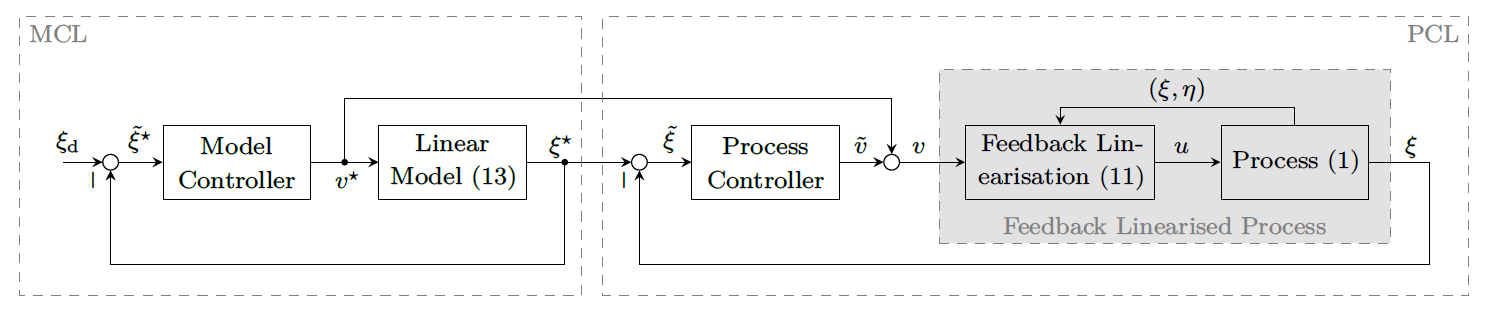
\includegraphics[width=0.8\textwidth]{imgs/section1/MFCEfficient.PNG}
    \caption{Simpler Model Following Control block diagram with model control loop process and control loop \cite{Tietze2023CruiseControl}.}
    \label{fig:Simpler_MFC_Control_Loop}
\end{figure}

To show how much this design is simpler, we can show \ref{fig:Simpler_MFC_Control_Loop_block} where the 
links between the MCL and the PCL are reduced and the linearization control law only lies into the PCL compared 
to the previous design.


\begin{figure}[htbp]
    \centering
    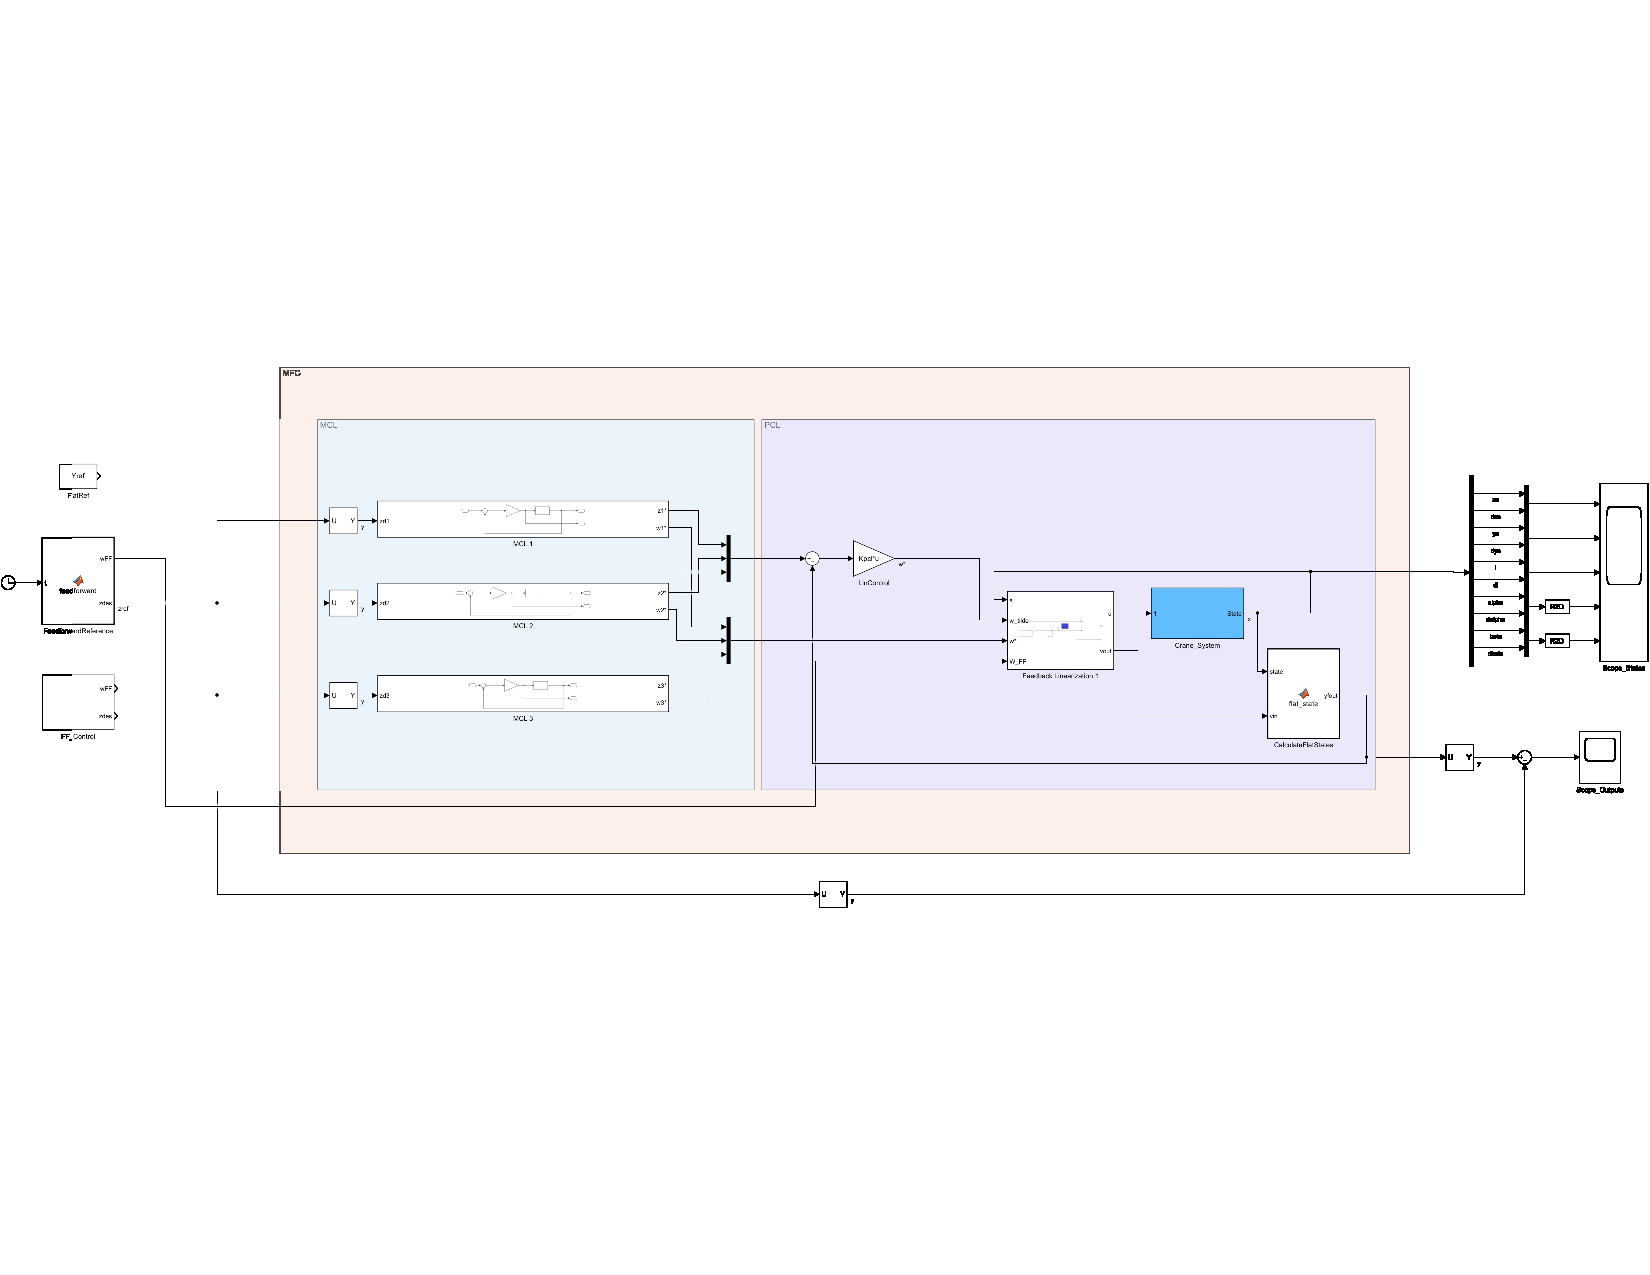
\includegraphics[width=0.5\textwidth]{imgs/section1/MFC_efficient_model.pdf}
    \caption{Simpler MFC Matlab Simulink implementation from \cite{Tietze2023CruiseControl}.}
    \label{fig:Simpler_MFC_Control_Loop_block}
\end{figure}

Now we can take a look on the meaning of the new architecture on the system equations.
The open-loop dynamics of the system are characterized by:

\begin{equation}
    \dot{\boldsymbol{\xi}} = A\boldsymbol{\xi} + B(\boldsymbol{y}_d^{(n)} + v) + \Delta(\boldsymbol{\xi}, t).
\end{equation}

A nominal model for the external dynamics is also presented:

\begin{equation}
    \dot{\boldsymbol{\xi}}^* = A\boldsymbol{\xi}^* + B(\boldsymbol{y}_d^{(n_\xi)} + v^*).
\end{equation}

The error dynamics, which are crucial for understanding deviations from the desired state, are expressed as:

\begin{equation}
    \dot{\tilde{\boldsymbol{\xi}}} = A\tilde{\boldsymbol{\xi}} + B(\tilde{v} + \Delta(\boldsymbol{\xi}, \eta, t)).
\end{equation}

The overall dynamics of the open-loop MFC system are described by:

\begin{align}
    \dot{\tilde{\boldsymbol{\xi}}}^* &= A\tilde{\boldsymbol{\xi}}^* + Bv^*, \\
    \dot{\tilde{\boldsymbol{\xi}}} &= A\tilde{\boldsymbol{\xi}} + B(\tilde{v} + \Delta(\boldsymbol{\xi}, t)).
\end{align}

Which is also way simpler than the previous design to understand and implement but lies on the idea of the previous 
one. 

\subsection{High Gain Control Comparison}

The High Gain Control law is formulated as:

\begin{equation}
    u = \frac{-a(\boldsymbol{\xi}) + K_\epsilon \boldsymbol{\xi}}{b(\boldsymbol{\xi})}.
\end{equation}

This well-known control law is used in only one loop, which would be the PCL in our case. It also handles the convergence of the model part to the desired state trajectory. This design is simpler to implement and the condition to encounter the perturbation is similar as seen in \cite{Willkomm2023MFC}. It leads to a more aggressive control even when the error doesn't need it for a rapid convergence but also to a high input work and the presence of the peaking phenomenon.

In classical high gain control, the gain \(K_\epsilon\) is typically chosen to be very large 
to ensure fast error convergence and the perturbation rejection. The cost of this method is a high
sensibility to all kind of errors between the desired trajectory and the real system trajectory. Especially 
when the initial condition is far away from the desired trajectory. The control input can reach very high values
at \(t=0\) to quickly reduce the error, this is the peaking phenomenon that can harm the system and can 
be avoided with the MFC strategy.

With this in mind, the High Gains approach is susceptible to the creation of the peaking phenomenon, 
potentially leading to:

\begin{itemize}
    \item Large, temporary deviations in the system's response.
    \item Actuator saturation, which can degrade performance or cause instability.
    \item Challenges in systems with fast dynamics or constrained states.
\end{itemize}

\subsection{Peaking Phenomenon and Advantages of MFC}

The peaking phenomenon is a critical limitation of high gain control, particularly in systems where transient 
performance is important. The large initial peaks in control signals can exceed actuator limits, leading to 
saturation and potential system failure. 

In contrast, MFC offers a robust alternative to mitigate the peaking phenomenon. 
MFC achieves this through several key mechanisms:

\begin{itemize}
    \item \textbf{Reduced Sensitivity to High Gains:} MFC does not rely solely on high gains to achieve 
    stability. Instead, the control loop assigned with predictable model dynamics (MCL) ensures that the system
    remains stable regarding only the desired trajectory without high gains which prevent from peaking due to
    initial condition far away from the desired trajectory. Its stability is easily ensured by the gain choice 
    taking out the perturbation issues from the model part to the process part.
    \item \textbf{Adaptive Error Compensation:} The error between the model and the real system is managed by the
    PCL, which can be tuned to respond to perturbations without the fear of high errors because the model is
    stabilised on the desired trajectory. Leaving the aggressive control to the PCL only when needed and 
    giving stability conditions on the time scaling factor \(\epsilon\) to encounter the perturbations.
\end{itemize}

Thus, MFC presents a compelling solution for systems where the peaking phenomenon poses a significant 
challenge, offering a balance between rapid convergence and robust transient performance.

Now that the MFC strategy has been presented, we can focus on the crane system and its dynamics to
implement the control law on it and compare the performances of those controllers to highlight the presence 
of the peaking phenomenon or not and also see the high input work needed for the High Gain control.


\newpage
% ---------------------------------------------------------------------------------------------------------------------------------------------------%
%                                                                                                                                                    %
%                                                                                                                                                    %
%                                                                                                                                                    %
% ---------------------------------------------------------------------------------------------------------------------------------------------------%

\section{Crane Overview}
\subsection{Crane Model}
The crane dynamic equations are computed as in \cite{Knierim2010Crane}. The trolley position \(\boldsymbol{r}_{t}(t)\) is considered as a time-dependent function:
\begin{equation}
    \textbf{r}_t(t) = \begin{bmatrix}
        a(t) & b(t) & 0
    \end{bmatrix}^T,
\end{equation}
where \(a(t)\) and \(b(t)\) are the positions of the trolley in the \(x\) and \(y\) directions.

In Figure~\ref{fig:Crane_Schema} we can see a schematic representation of the crane system. The load is suspended 
from the trolley by a cable of length \(l(t)\), which can vary over time. The angles \(\alpha(t)\) and 
\(\beta(t)\) represent the swing of the load in the \(x\) and \(y\) directions, respectively.

\begin{figure}[htbp]
    \centering
    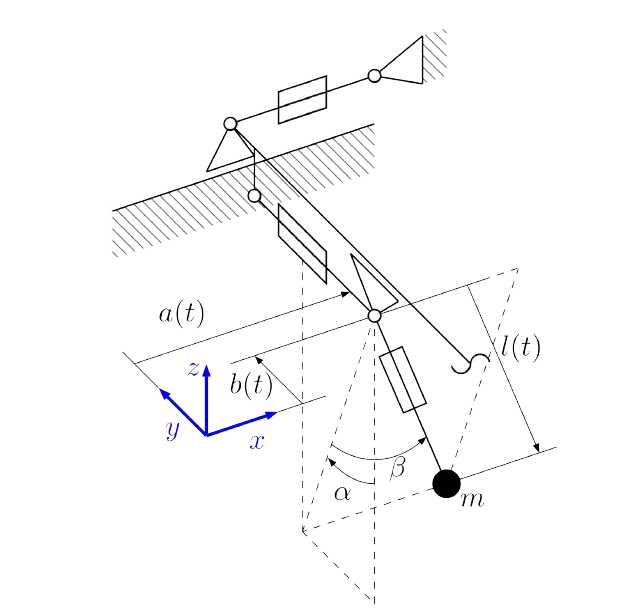
\includegraphics[width=0.6\textwidth]{imgs/section1/3DimCranSchem.PNG}
    \caption{Schematic representation of the crane system with trolley and load positions.}
    \label{fig:Crane_Schema}
\end{figure}

Then, using the cardan angles of the pivot point \(\alpha\) and \(\beta\), one can express the 
position of the load, which will be the output of the system as \(\textbf{y}(t)\) given by:

\begin{equation}
    \textbf{y}(t) = \begin{bmatrix}
        a(t) + l(t)S_\beta \\
        b(t) + l(t)C_\beta S_\alpha \\
        -l(t)C_\beta C_\alpha
    \end{bmatrix},
\end{equation}
with the notations \(S_\gamma = \sin(\gamma)\) and \(C_\gamma = \cos(\gamma)\).

The state \([a(t), b(t), l(t)]\) is taken to have its second derivative directly controlled by the input.
The angles \(\alpha(t)\) and \(\beta(t)\)  are considered internal states of the system. They are not directly controlled but are influenced by the motion of the trolley and the length of the cable.
We need to find their dynamics to have a complete state-space representation of the system. The utilisation of the
generalized coordinates vector \(\boldsymbol{\theta} = \left[ \alpha \; \beta \right]^T\) is to be derived
and used in the Newton-Euler equation of the load system. 

The Jacobian of the crane over the generalized coordinates is:

\begin{equation}
    \boldsymbol{J}_{l}(t) = \frac{\partial \boldsymbol{y}(t)}{\partial \boldsymbol{\theta}} = \begin{bmatrix}
        0                       & l(t)C_\beta \\
        l(t)C_\beta C_\alpha   & -l(t)S_\beta S_\alpha \\
        l(t)C_\beta S_\alpha   & l(t)S_\beta C_\alpha
    \end{bmatrix}.
\end{equation}

The velocity and acceleration of the load are given by:
\begin{align}
    \dot{\boldsymbol{y}} &= \boldsymbol{J}_{l}(t) \dot{\theta} + \underbrace{ \left. \frac{\partial \boldsymbol{y}}{\partial t} \right\|_{\theta=cst}}_{\bar{\dot{\boldsymbol{y}}}(t)}, \\
    \ddot{\boldsymbol{y}} &= \boldsymbol{J}_{l}(t) \ddot{\theta} + \underbrace{\frac{d\boldsymbol{J}_{l}(t)}{dt} \cdot \dot{\boldsymbol{\theta}} + \frac{d\bar{\dot{\boldsymbol{y}}}(t)}{dt}}_{\bar{\ddot{\boldsymbol{y}}}(t)}.
\end{align}

The mass matrix of the load with mass \(m\) is taken as punctual and given by:
\begin{equation}
    \boldsymbol{M} = \boldsymbol{I}_3 m
\end{equation}

where \(\boldsymbol{I}_3\) is the \(3 \times 3\) identity matrix. The Newton-Euler equation is 
applied to derive the equations of motion:

The distribution matrix \(\boldsymbol{Q}\) in the Newton-Euler equation represents the direction of 
the reaction force \(\boldsymbol{q}_r\) between the load and the trolley. Since the reaction 
force can only act along the rope, \(\boldsymbol{Q}\) is defined as the unit vector in the 
direction of the rope:

\begin{equation}
    \boldsymbol{Q} = \frac{\boldsymbol{r}_t(t) - \boldsymbol{r}_l(t)}{\left\|\boldsymbol{r}_t(t) - \boldsymbol{r}_l(t)\right\|} = \begin{bmatrix}
    S_\beta \\
    C_\beta S_\alpha \\
    C_\beta C_\alpha
    \end{bmatrix}.
\end{equation}

Here, \(\boldsymbol{r}_t(t)\) and \(\boldsymbol{r}_l(t)\) are the position vectors of the 
trolley and the load, respectively. The matrix \(\boldsymbol{Q}\) effectively projects the 
reaction force \(\boldsymbol{q}_r\) along the rope, ensuring that the force is applied in the correct 
physical direction. 


\begin{equation}
    \label{eq:Newton_Euler}
    \boldsymbol{M} \boldsymbol{J}_{l}(t) \cdot \ddot{\boldsymbol{\theta}} = -\boldsymbol{M} \ddot{\boldsymbol{y}}(t) + \boldsymbol{q}_{e} + \boldsymbol{Q} \boldsymbol{q}_{r}
\end{equation}    

where \(\boldsymbol{q}_{e}\) denotes the vector of external forces, primarily due to gravity. 
Hence \(\boldsymbol{Q}^T\boldsymbol{J}_{l}(t) = \boldsymbol{J}_{l}(t)^T\boldsymbol{Q}= 0\) and 
multiplying by \(\boldsymbol{J}_{l}(t)^T\), we eliminate the reaction forces \(\boldsymbol{q}_r\) 
in \ref{eq:Newton_Euler}, knowing that \(\boldsymbol{M} = \boldsymbol{I}_3m\) the equation of motion in 
generalized coordinates \(\boldsymbol{\theta}\) reads:

\begin{equation}
    \label{eq:equation_of_motion_generalized_coordinates}
    m \cdot \boldsymbol{J}_{l}(t)^T\boldsymbol{J}_{l}(t)\cdot \ddot{\boldsymbol{\theta}} = - m \cdot\boldsymbol{J}_{l}(t)^T \: \bar{\ddot{\boldsymbol{y}}}(t) \; + \; m \cdot \boldsymbol{J}_{l}(t)^T\boldsymbol{g}
\end{equation}

where \(\boldsymbol{g} = \begin{bmatrix} 0 & 0 & -g\end{bmatrix}^T\) denotes the gravity vector, 
and it is easy to remark that the equation \ref{eq:equation_of_motion_generalized_coordinates} is 
independent of the load mass \(m\).

The input is the same as in the simulation and real crane experimentation, directly driving the 
\(\begin{bmatrix}\ddot{a}(t) & \ddot{b}(t) & \ddot{l}(t)\end{bmatrix}\) coordinates. The complete 
dynamics of the crane plant system are given by the following non-linear vectorial second-order differential 
equation \cite{Knierim2010Crane}:

\begin{align}
    \left\{ \begin{array}{ll}
    \ddot{a}(t) &= u_1, \\
    \ddot{b}(t) &= u_2, \\
    \ddot{l}(t) &= u_3, \\
    \ddot{\alpha}(t) &= \frac{1}{l(t) C_{\beta}} \left(2 \dot{\alpha} \dot{\beta} S_{\beta} l(t) - 2 \dot{l}(t) \dot{\alpha} C_{\beta} - S_{\alpha} g - C_{\alpha} u_2\right), \\
    \ddot{\beta}(t) &= \frac{1}{l(t)} \left(-C_{\alpha} S_{\beta} g - S_{\beta} C_{\beta} \dot{\alpha}^2 l(t) - 2 \dot{l}(t) \dot{\beta} + S_{\beta} S_{\alpha} u_2 - C_{\beta} u_1\right).
    \end{array}
    \right.
\end{align}

The system can now be written in normal form:

\begin{align*}
    \dot{\boldsymbol{x}} &= \boldsymbol{f}(\boldsymbol{x}) + \boldsymbol{g}(\boldsymbol{x})\boldsymbol{u}, \\
    \boldsymbol{y} &= \boldsymbol{h}(\boldsymbol{x}),
\end{align*}

where the state vector \(\boldsymbol{x}(t)\) is:

\begin{align*}
    \boldsymbol{x}(t) &= (x_i(t))_{1\le i\le 10} \\
    &= \begin{pmatrix} a(t) & \dot{a}(t) & b(t) & \dot{b}(t) & l(t) & \dot{l}(t) & \alpha(t) & \dot{\alpha}(t) & \beta(t) & \dot{\beta}(t)\end{pmatrix}^T.
\end{align*}

\subsection{Feedback Linearization and Dynamic Extension}

The feedback linearization applied directly to the crane equation results in internal dynamics. To address this, a dynamic extension is implemented as in \cite{Noack2020} by introducing a virtual control input:
\begin{align}
    \ddot{\nu} &= w_3, \\
    u_3 &= \psi(\boldsymbol{x}, \nu),
\end{align}
where \(u_3\) is computed such that \(\forall t \ge 0, \quad \ddot{y}_3(t) - \nu(t) = 0\).

With the crane system, the relative degrees of the outputs \([y_1, y_2, y_3]^T\) are \([2, 2, 2]^T\), leading to internal dynamics. The dynamic extension increases the relative degrees to \([4, 4, 4]^T\).

By applying the following transformation to each output \(y_i\) for \(i \in \{1, 2, 3\}\):
\begin{equation}
\boldsymbol{\xi}_i = \boldsymbol{T}_i(\boldsymbol{x}) = \begin{bmatrix} y_i \\ \dot{y}_i \\ \ddot{y}_i \\ y^{(3)}_i \end{bmatrix},
\end{equation}
the system is divided into three decoupled subsystems in Byrnes-Isidori form:
\begin{equation}
\label{eq:flat_sys_reduced}
\forall i \in \{1, 2, 3\} :
\left\{
\begin{aligned}
  \dot{\boldsymbol{\xi}_i} &= \boldsymbol{A} \boldsymbol{\xi}_i + \boldsymbol{B} \big(a_i(\boldsymbol{\xi}) + b_i(\boldsymbol{\xi})u\big), \\
  \boldsymbol{y}_i &= \boldsymbol{C} \boldsymbol{\xi}_i.
\end{aligned}
\right.
\end{equation}

\section{Implementation on a Crane Simulation}
All of the control law has been defined, we can test its performances on a crane system but first, it will be run through a simulation on Matlab Simulink. 
The analysis is conducted in three situations: stabilizing on a setpoint, and then setpoint and trajectory tracking. The goal is to observe the presence or not of the peaking phenomenon depending on the initial conditions of the Model Control Loop and we will verify just on the simulation the exact same behavior between the original MFC and the simpler design.

% ===============================================================================================%
%                                                                                               %
%                                                                                               %
% ===============================================================================================%


\section{Results}
\subsection{Simulation Results}

The simulation results have been obtained using the Simulink model shown in Figure~\ref{fig:Simulink_MFC_Loop} and 
the environment provided in the code in appendix \ref{app:Matlab_environement}.


\begin{figure}[htbp]
    \centering
    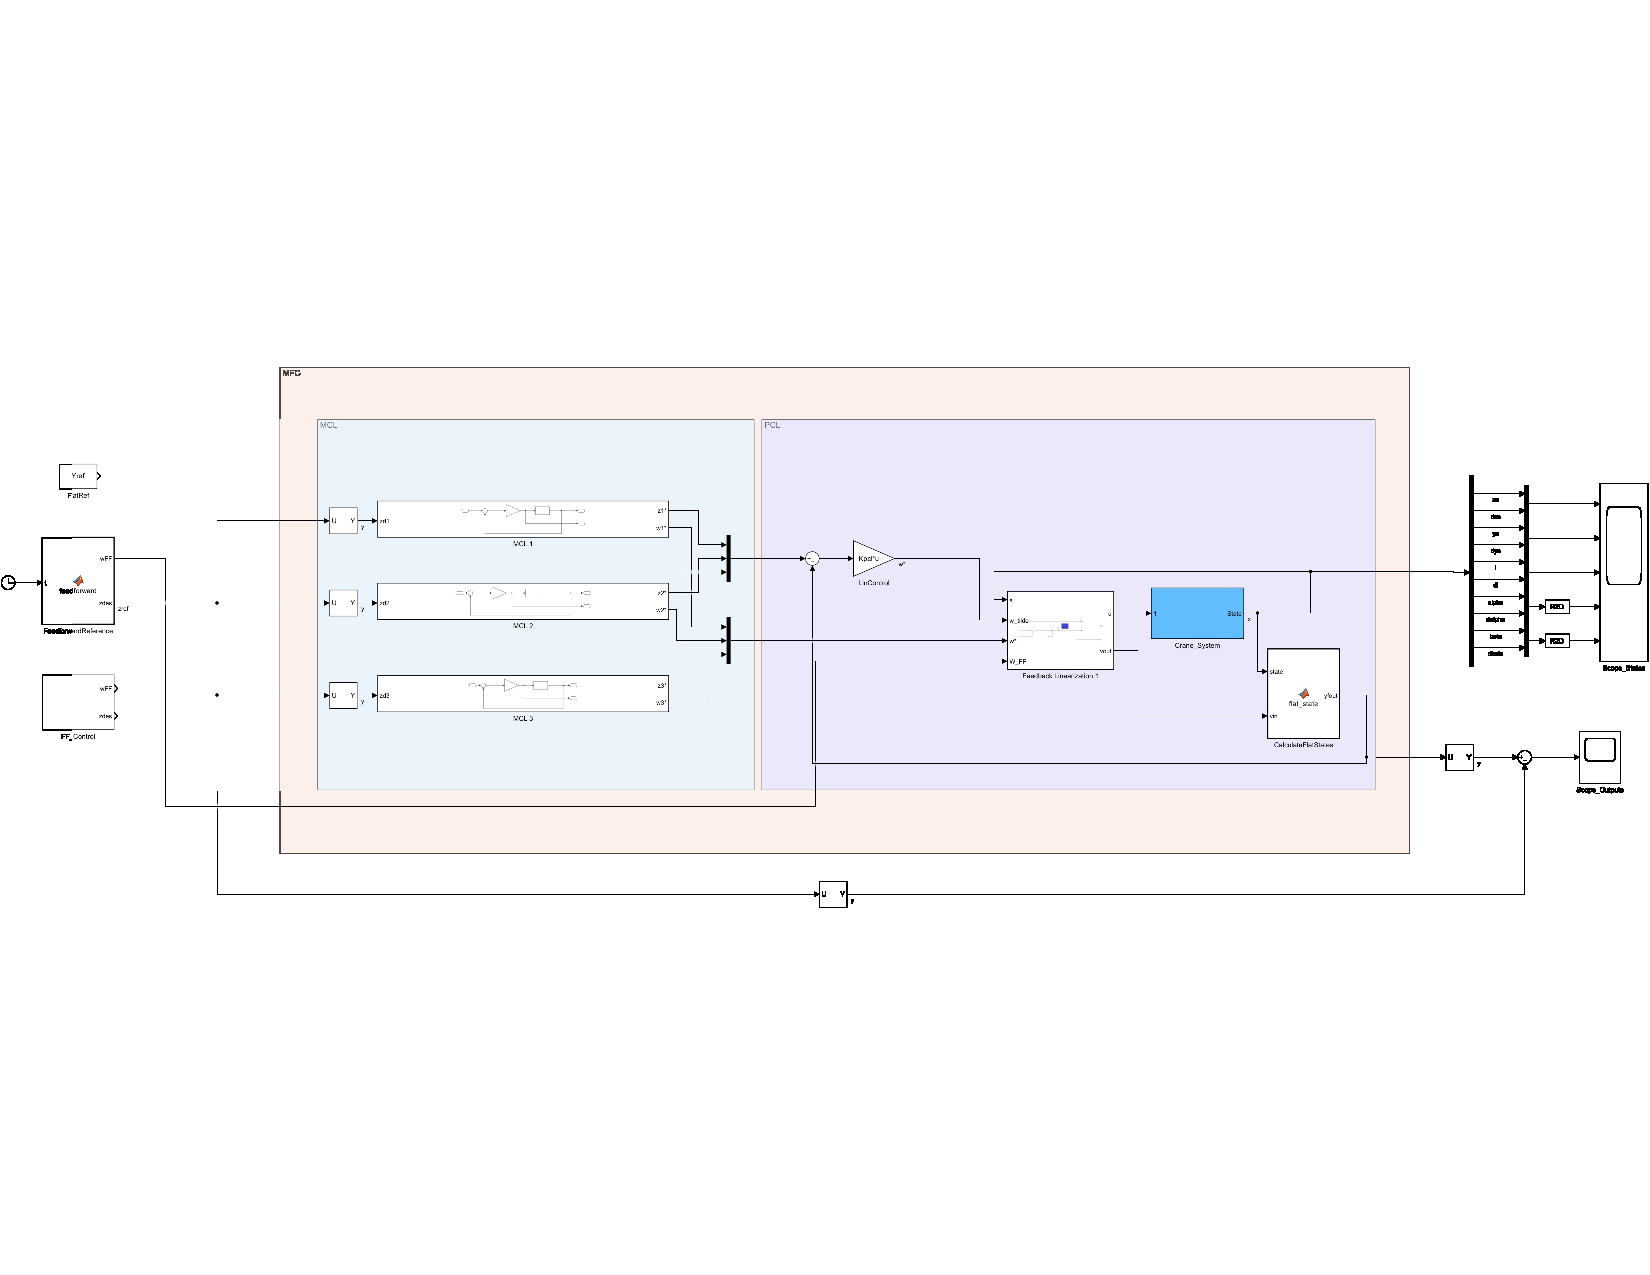
\includegraphics[width=0.9\linewidth]{imgs/section1/MFC_efficient_model.pdf}
    \caption{Simulink model of the MFC loop.}
    \label{fig:Simulink_MFC_Loop}
\end{figure}

The model includes both the MFC and High Gain control strategies for comparison. The crane system is 
represented with its full nonlinear dynamics, and the controllers are implemented with the designs 
discussed earlier.

To show the efficacy of the MFC strategy, we will compare the performances of both the MFC and High Gain control 
strategies in a trajectory tracking task. The desired trajectory for the load is shown 
in Figure~\ref{fig:Desired_Trajectory}. The load at its initial position won't be at the desired trajectory
such that : 

\begin{equation}
    \boldsymbol{\xi}(0) \neq \boldsymbol{\xi}_d(0)
\end{equation}

Which will create a high error at the beginning of the trajectory tracking and will highlight the 
peaking phenomenon for the High Gain control strategy.

\begin{figure}[htbp]
    \centering
    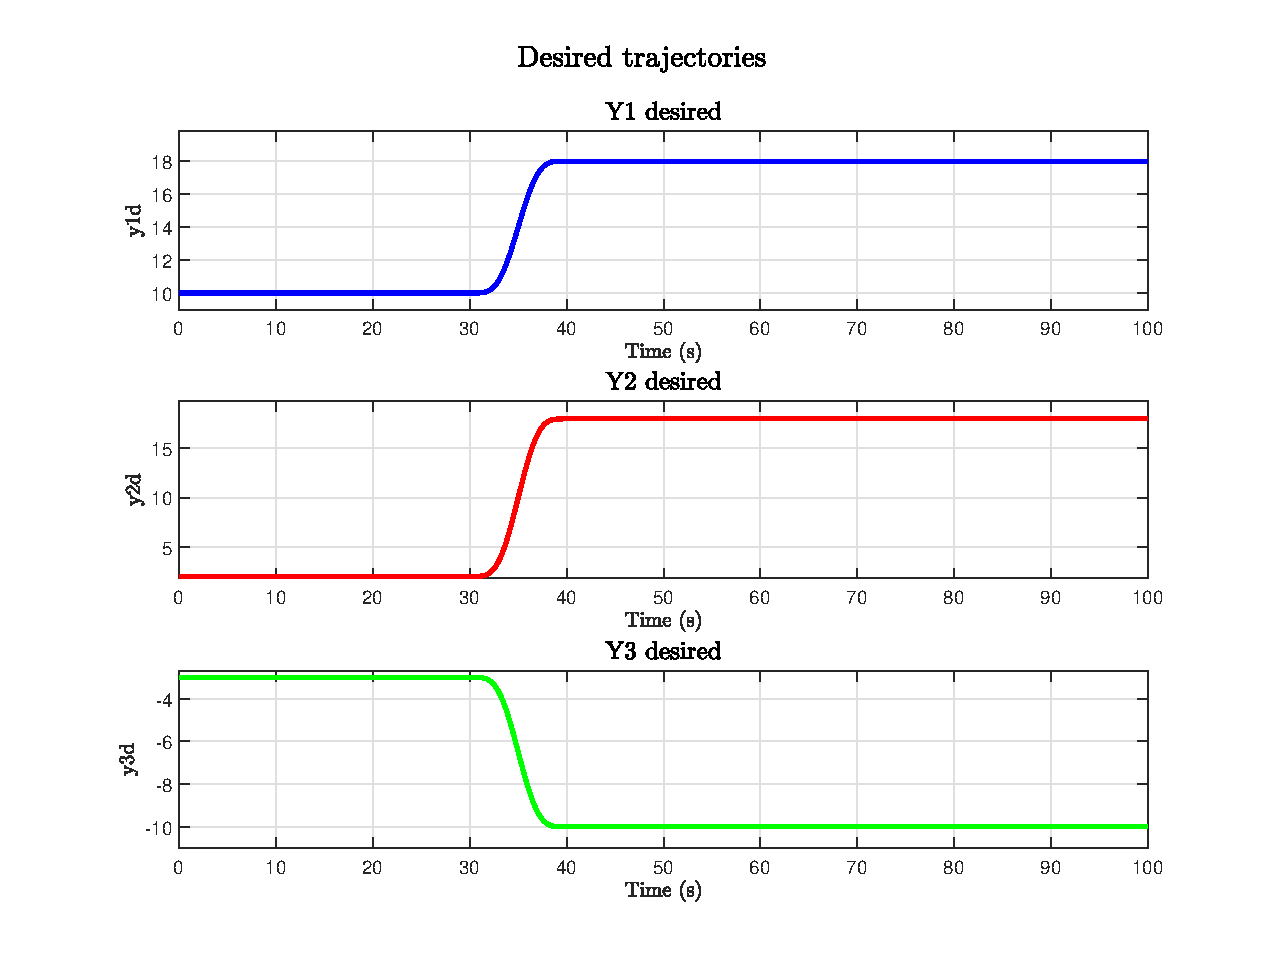
\includegraphics[width=0.75\linewidth]{imgs/section1/desiredTraj.eps}
    \caption{Desired trajectories of the load.}
    \label{fig:Desired_Trajectory}
\end{figure}

The Figure~\ref{fig:XY_Trajectory} shows the desired and actual (only for MFC) trajectories of the load in 
the \(xy\)-plane to get a better view of the trajectory tracking and the difference at the initial time.

\begin{figure}[htbp]
    \centering
    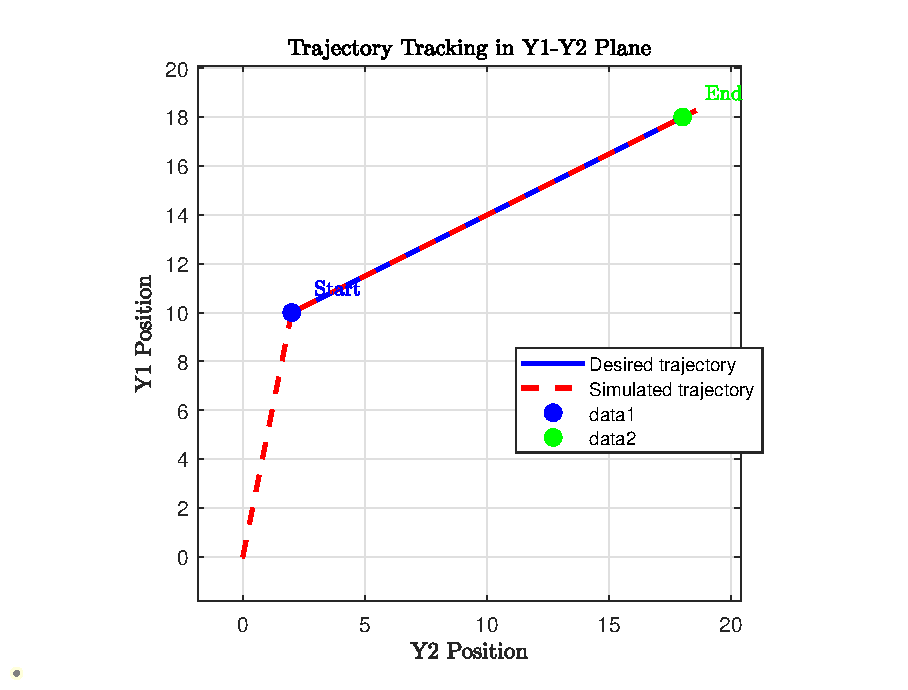
\includegraphics[width=0.8\linewidth]{imgs/section1/XYTrajectory.eps}
    \caption{Difference between desired states and model states.}
    \label{fig:XY_Trajectory}
\end{figure}

The next two figures Fig~\ref{fig:Input_High_Gain} and Fig~\ref{fig:Input_MFC} show the control inputs for 
both strategies.

\begin{figure}[htbp]
    \centering
    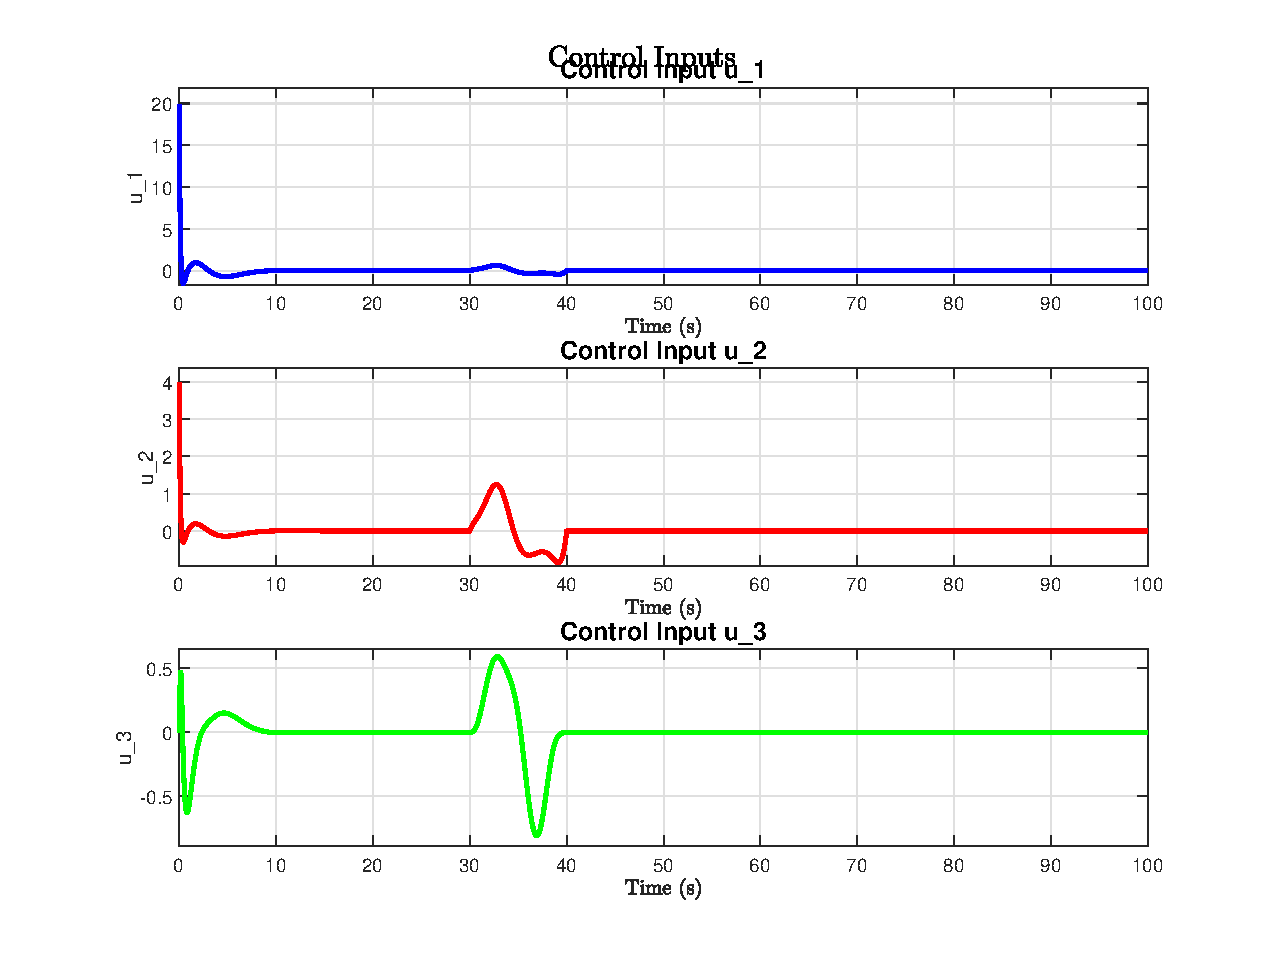
\includegraphics[width=0.8\linewidth]{imgs/section1/u_HG.eps}
    \caption{Input for set-point tracking using high-gain control.}
    \label{fig:Input_High_Gain}
\end{figure}

\begin{figure}[htbp]
    \centering
    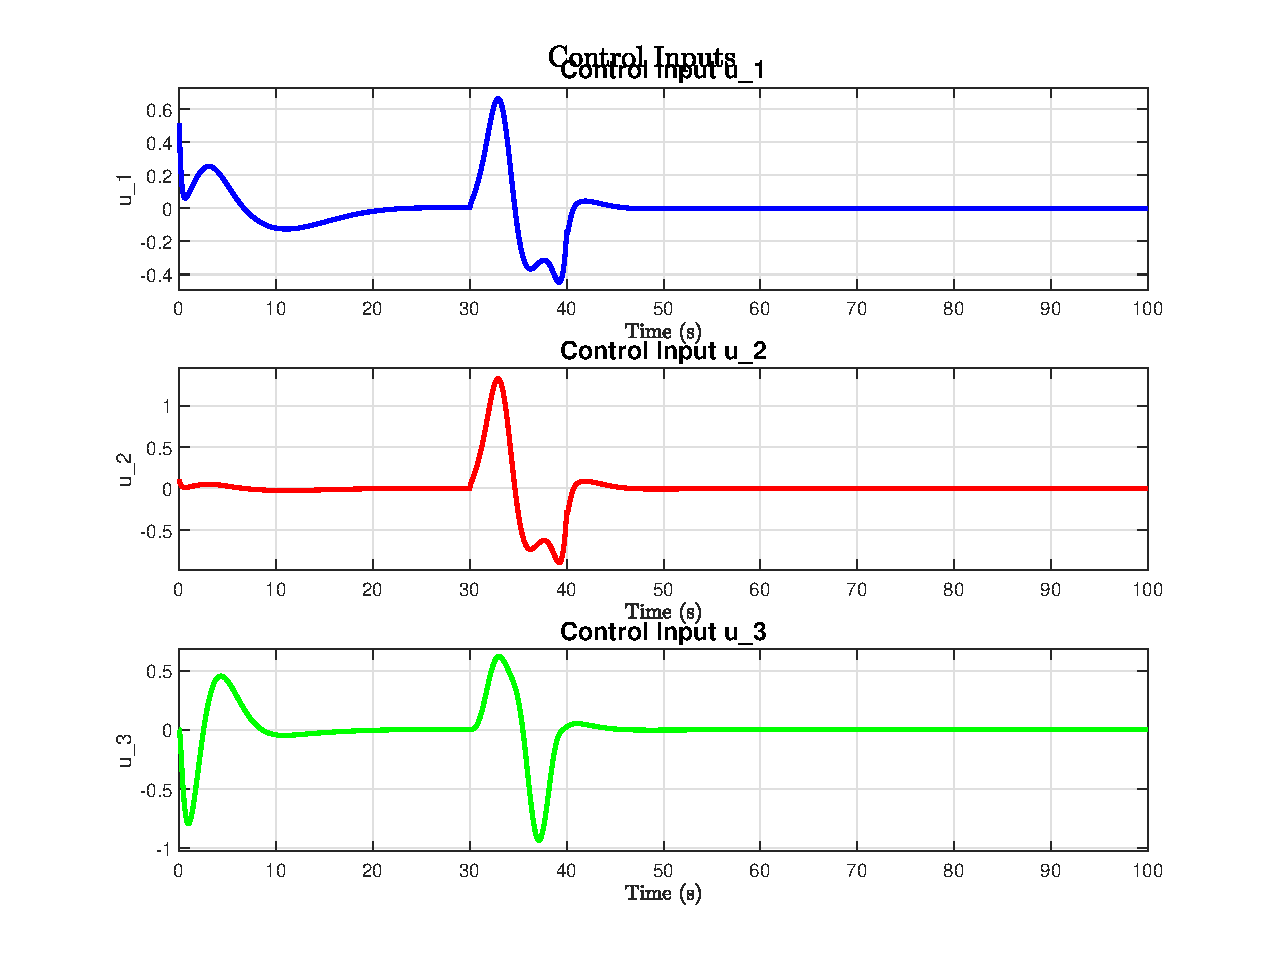
\includegraphics[width=0.8\linewidth]{imgs/section1/u_efficientMFC_Good_CI.eps}
    \caption{Input for set-point tracking using MFC.}
    \label{fig:Input_MFC}
\end{figure}

One can see that behaviors of both controllers aligns well with the predictions with a peak at \(t = 0\) for 
the High Gain control strategy and a reasonable input for the MFC strategy.

Now we can focus on the real plant experiment to see if the theory holds in a real environment with the environment
D-Space control Desk.

\newpage
\subsection{Real Plant Experiment}

We can see on figures~\ref{fig:Trolley_Zoom}, \ref{fig:X_Motor_Zoom} 
and \ref{fig:Y_Motor_Zoom} the the real plant crane system used for the
experimentation.

All of the control have been implemented on a 2011 version of Matlab Simulink
then compiled on D-space control desk. I won't go into the details of the
implementation on D-space because it is not the goal of this report but here 
in appendix \ref{app:Dspace_implementation} is an overview of the steps needed
to launch the control on the real plant.

\begin{figure}[htbp]
    \centering
    \rotatebox{270}{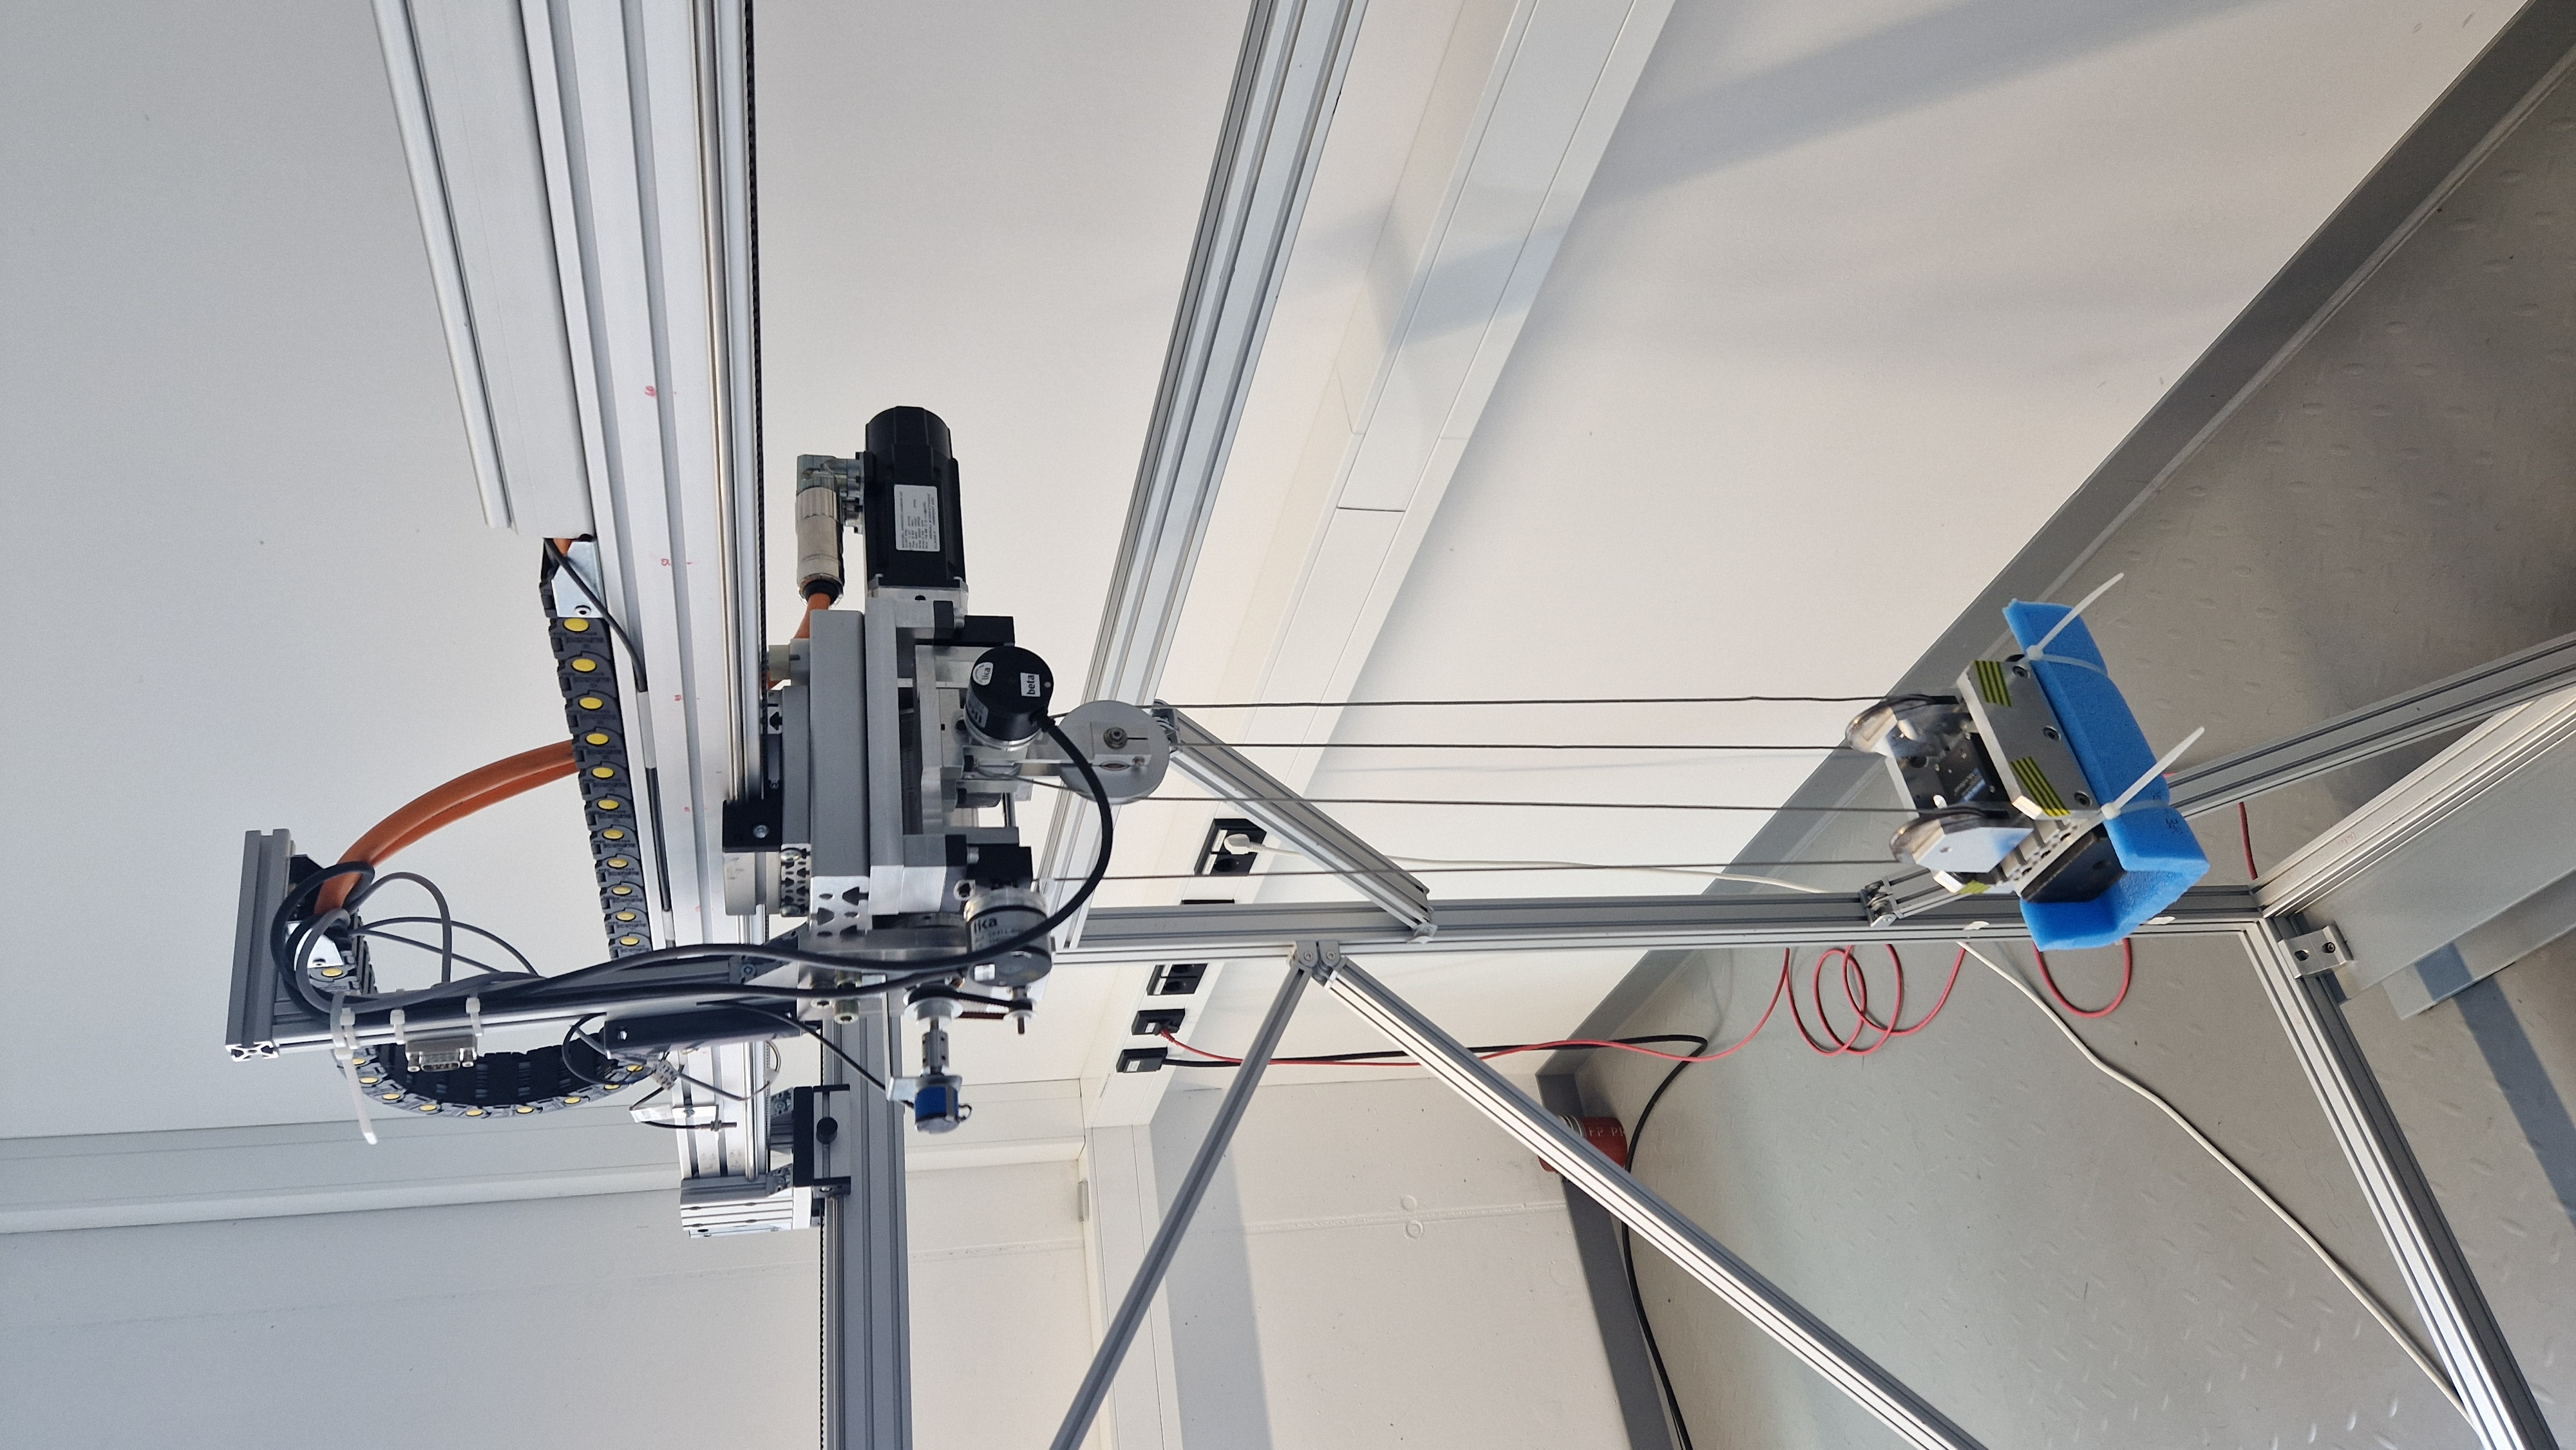
\includegraphics[width=0.5\linewidth]{imgs/section1/Trolley.jpg}}
    \caption{Zoom on the crane's trolley.}
    \label{fig:Trolley_Zoom}
\end{figure}

\begin{figure}[htbp]
    \begin{subfigure}{0.5\textwidth}
        \centering
        \rotatebox{270}{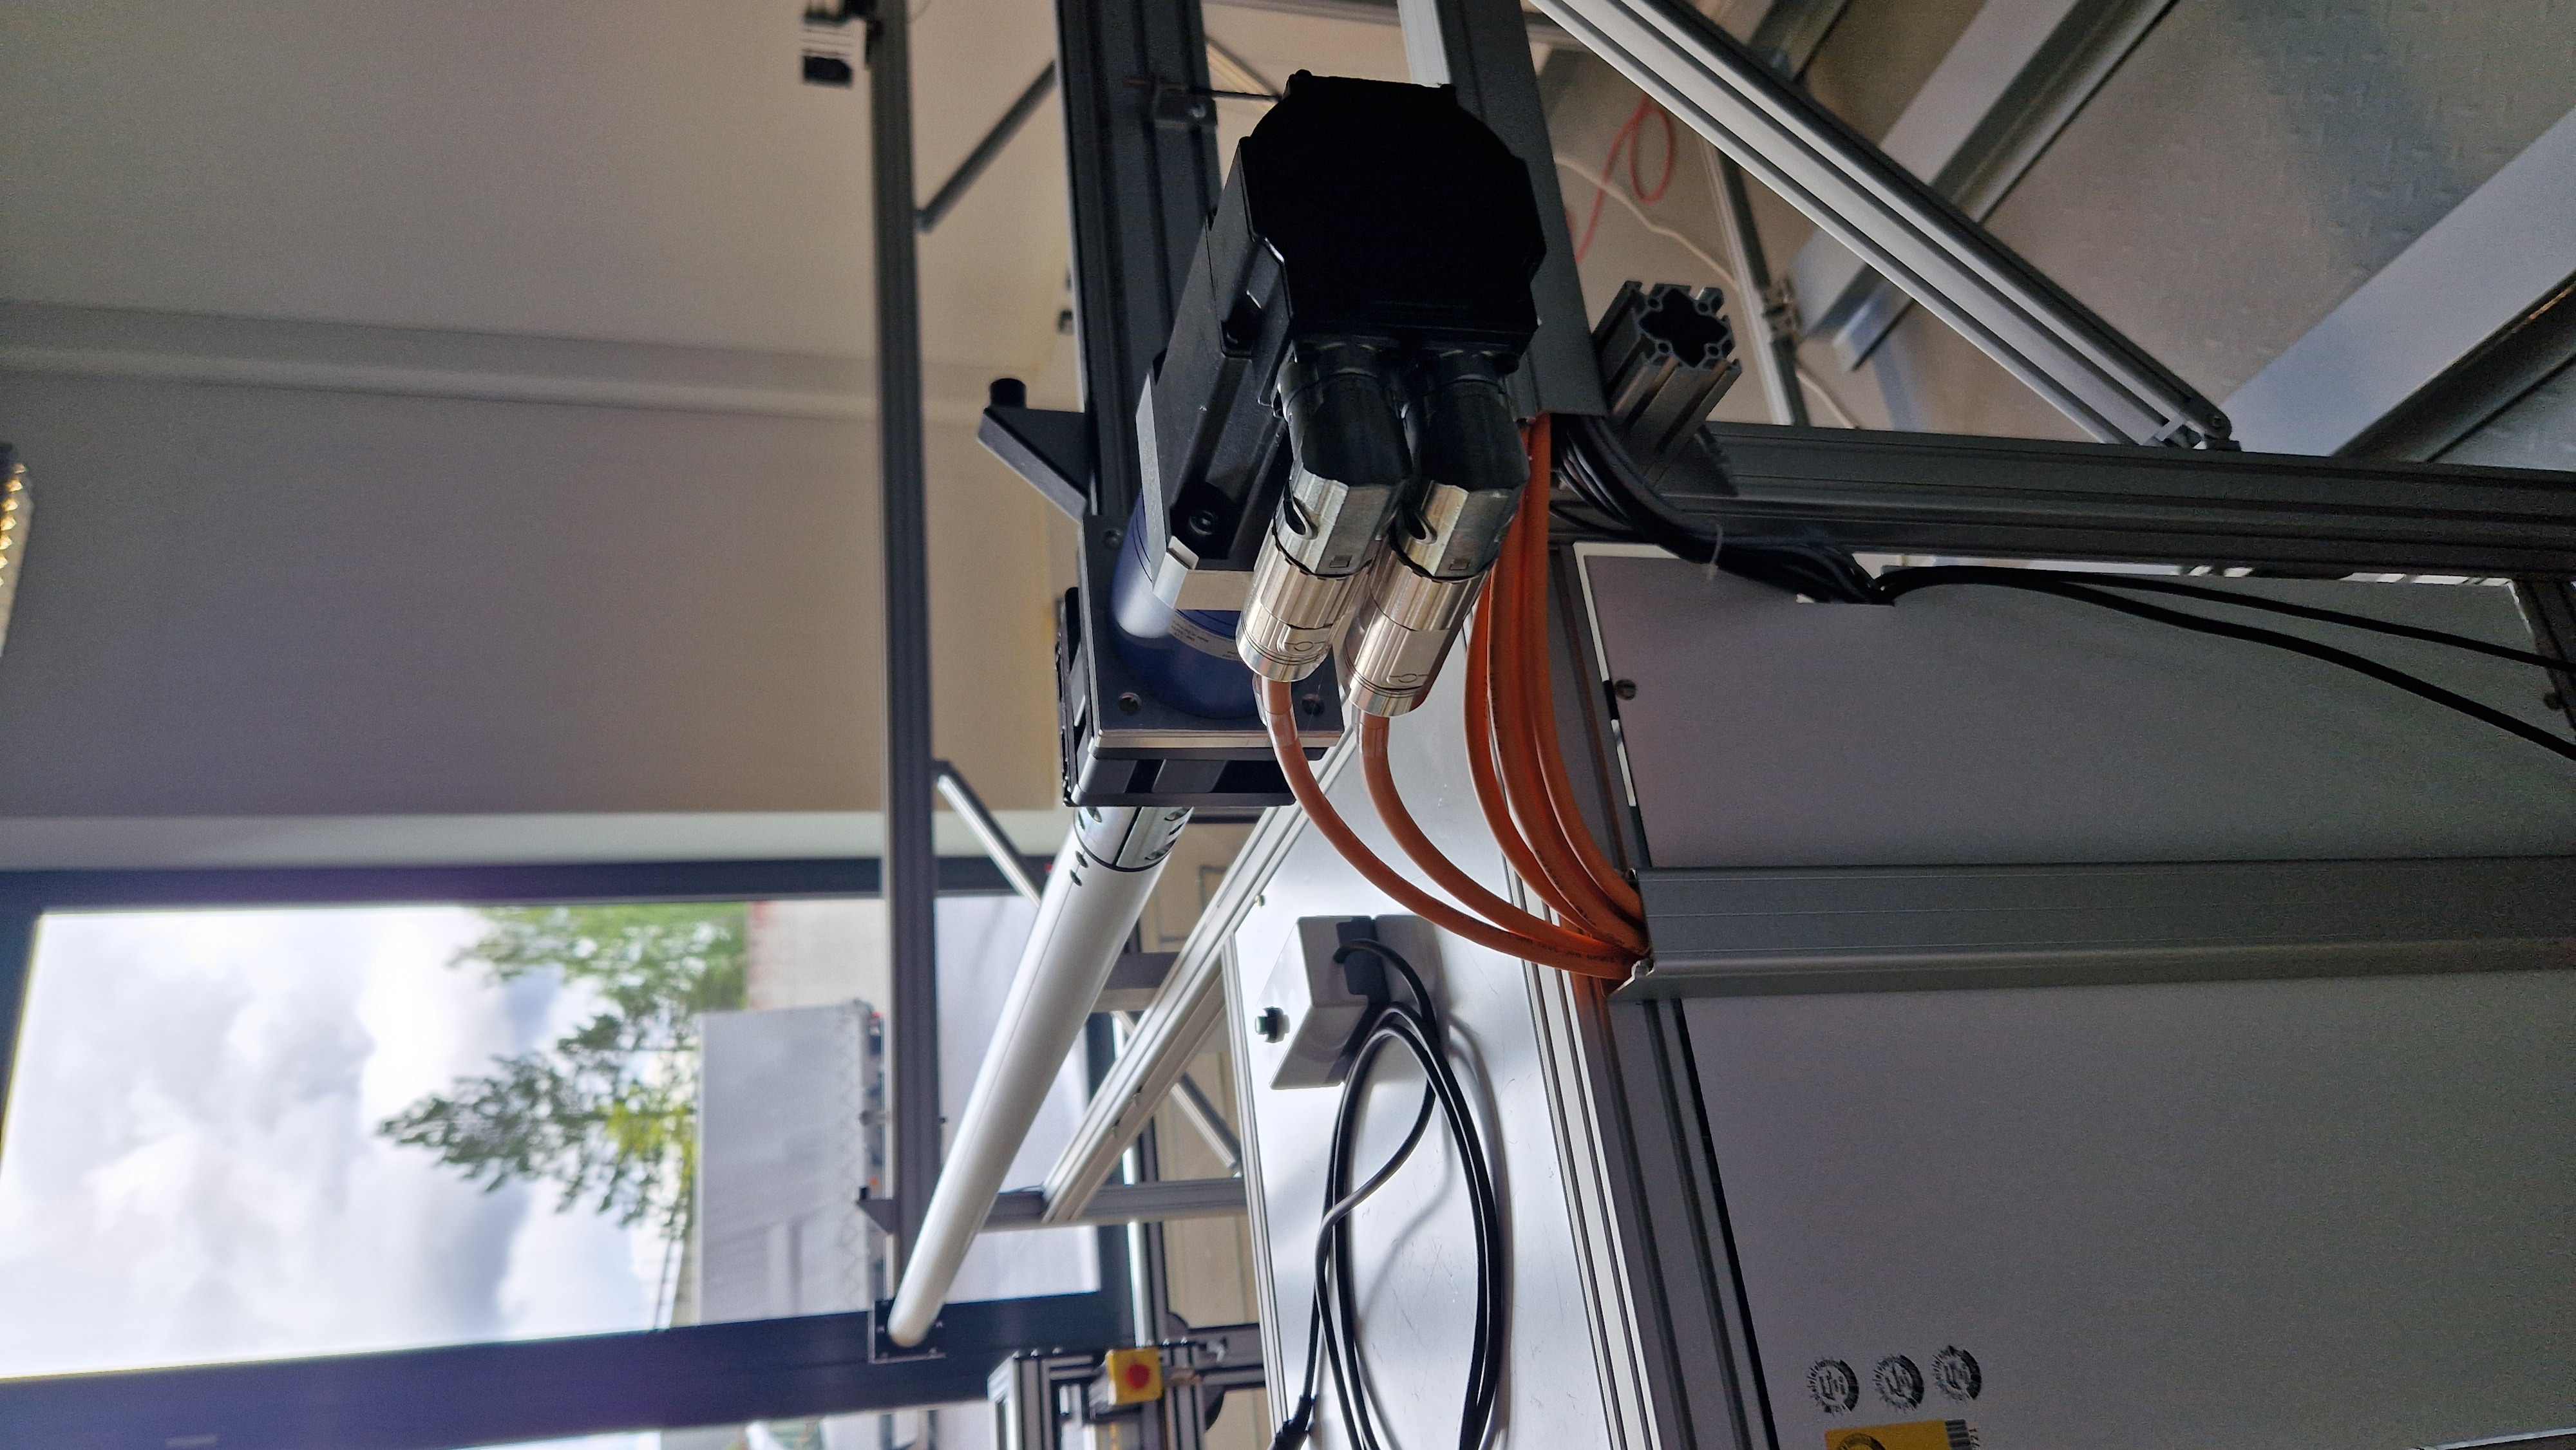
\includegraphics[width=\linewidth]{imgs/section1/Xmot.jpg}}
        \caption{Zoom on X motor.}
        \label{fig:X_Motor_Zoom}
    \end{subfigure}
    \hfill
    \begin{subfigure}{0.5\textwidth}
        \centering
        \rotatebox{270}{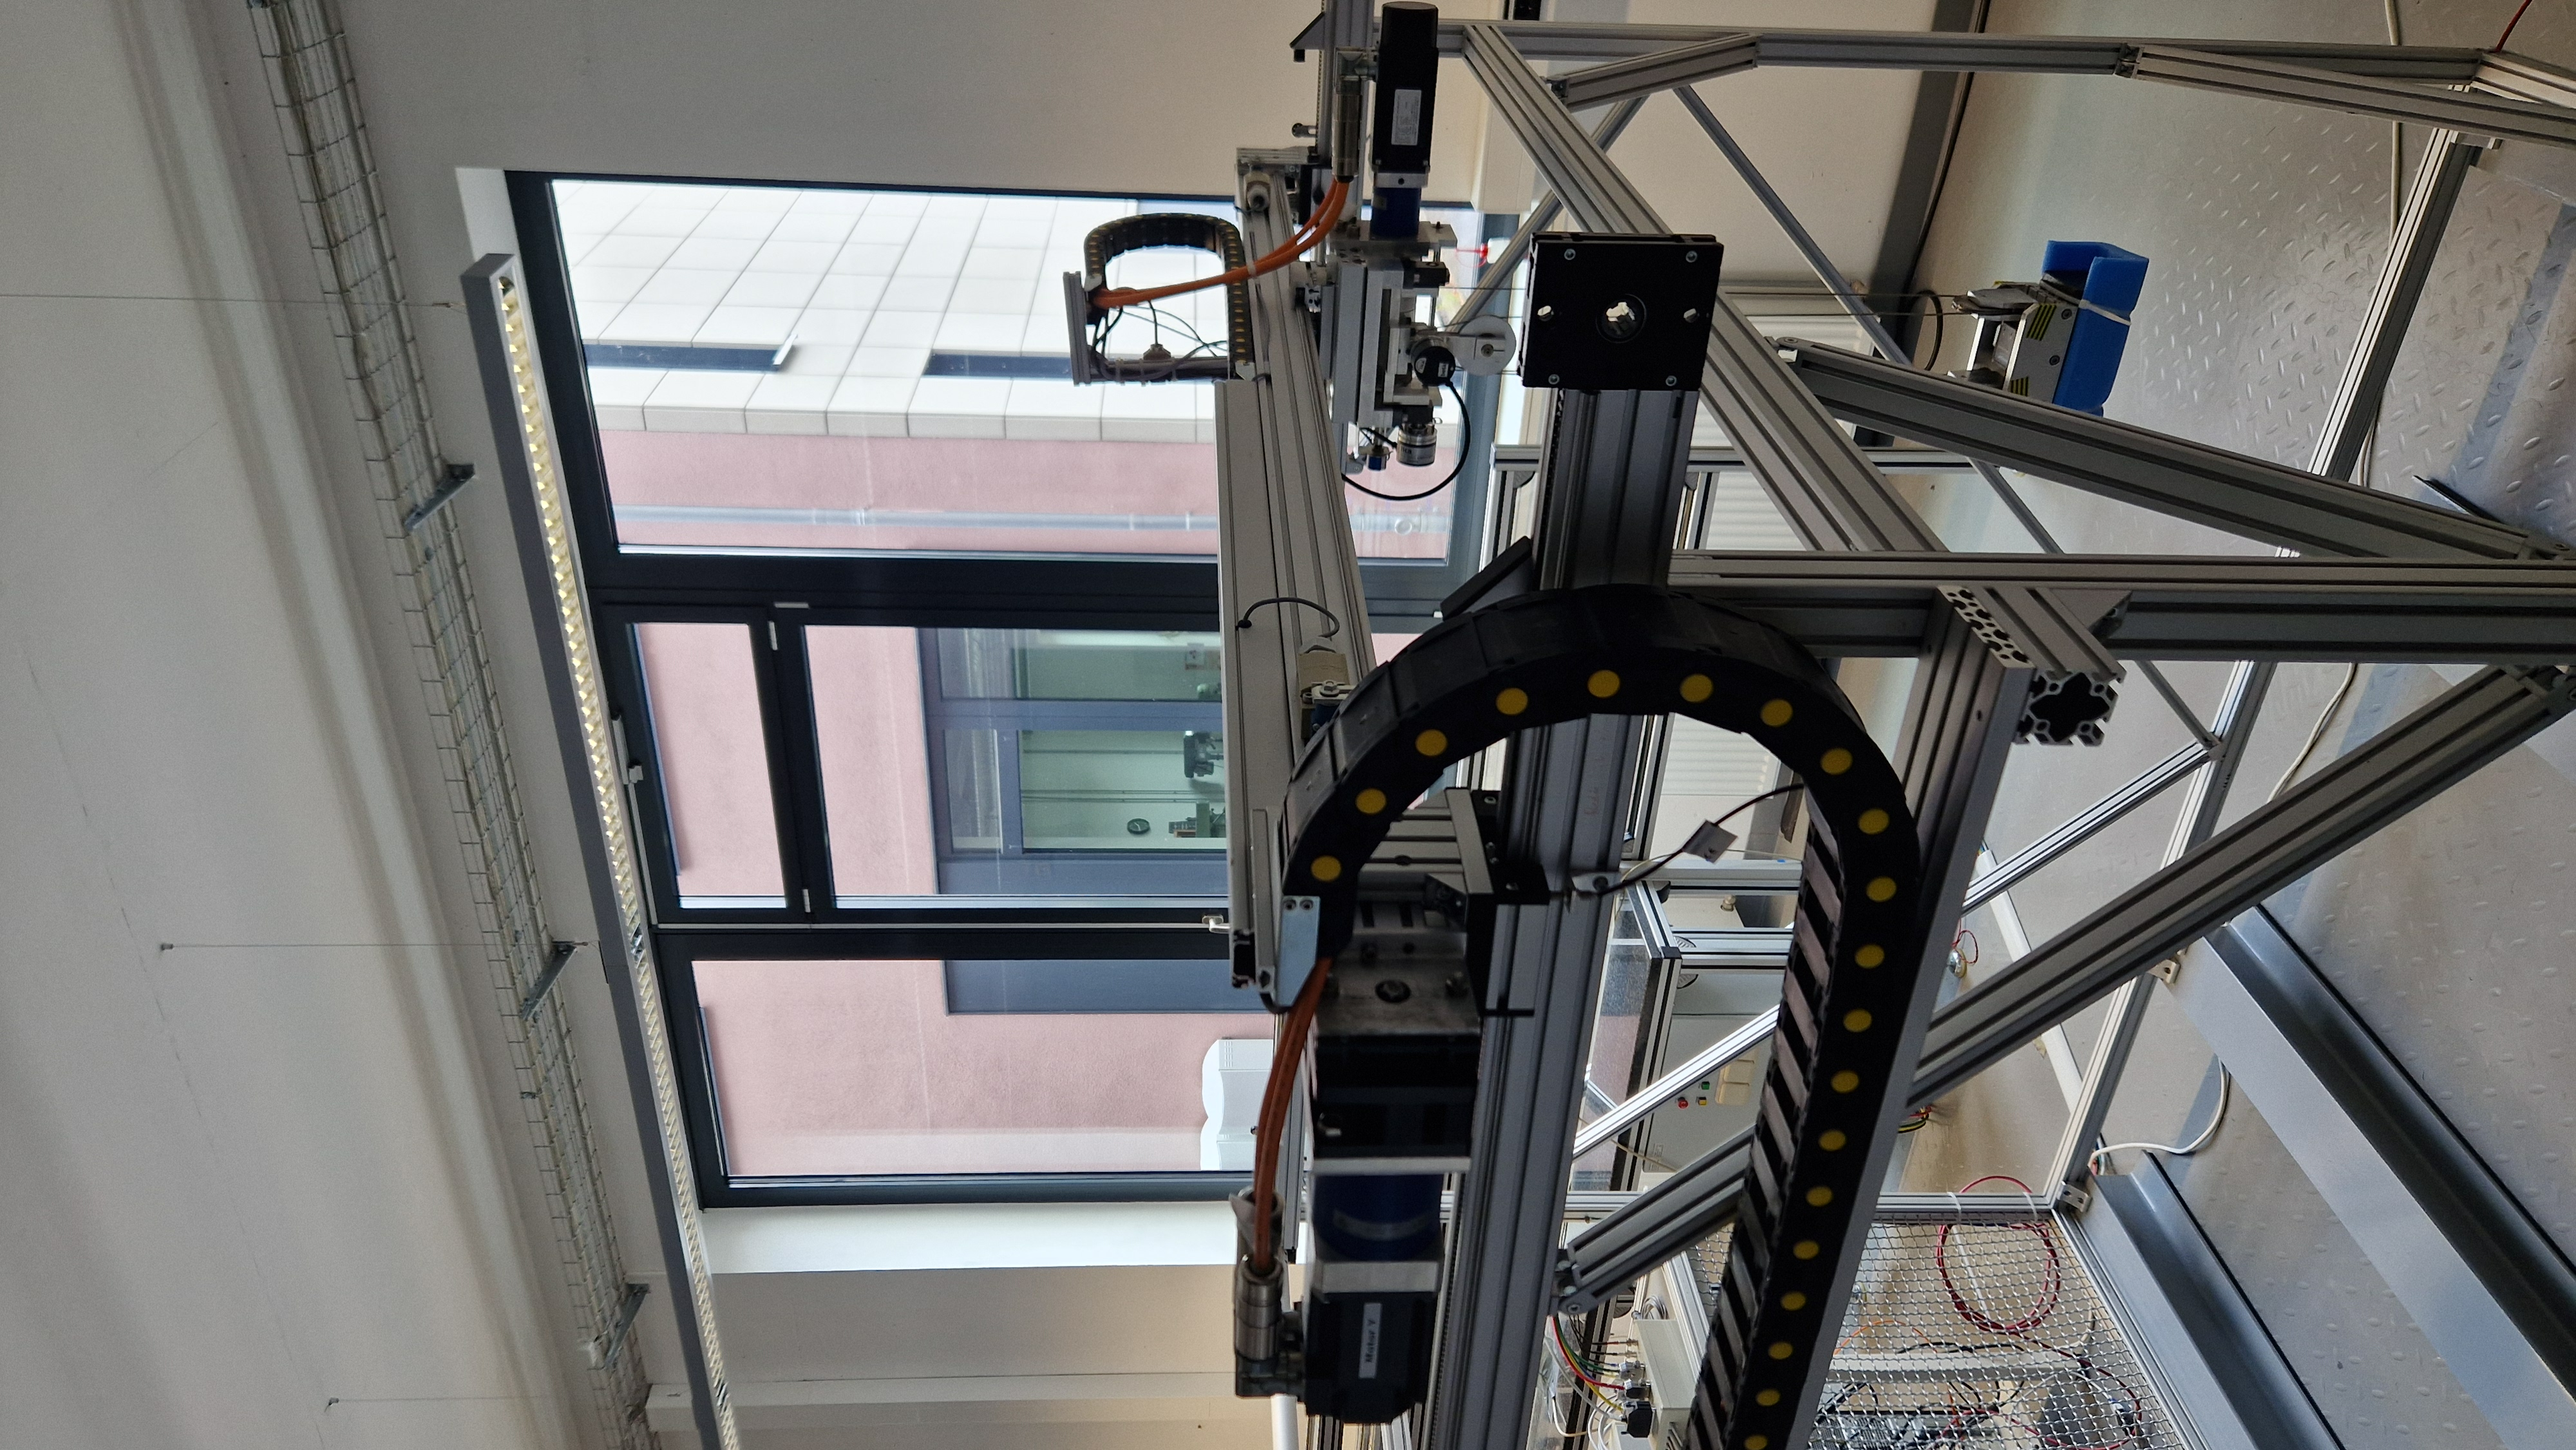
\includegraphics[width=\linewidth]{imgs/section1/Ymot.jpg}}
        \caption{Zoom on Y motor.}
        \label{fig:Y_Motor_Zoom}
    \end{subfigure}
    \caption{Zoom on the crane's X and Y motors.}
    \label{fig:Motors_Zoom}
\end{figure}


With this crane system, we implemented the same kind of trajectory to 
test the peaking phenomenon. The values aren't the same but method remains.
The figures ~\ref{fig:Real_PLant_without_Peaking} and 
~\ref{fig:Real_Plant_with_Peaking} highlight the peaking phenomenon
presence in the MFC control when the initial condition of the model aren't
taken close enough to the desired trajectory, the control behaves like a
High Gain and the high input work is present at the beginning as we can 
see on figure ~\ref{fig:Real_Plant_with_Peaking}.


\begin{figure}[htbp]
  \centering
  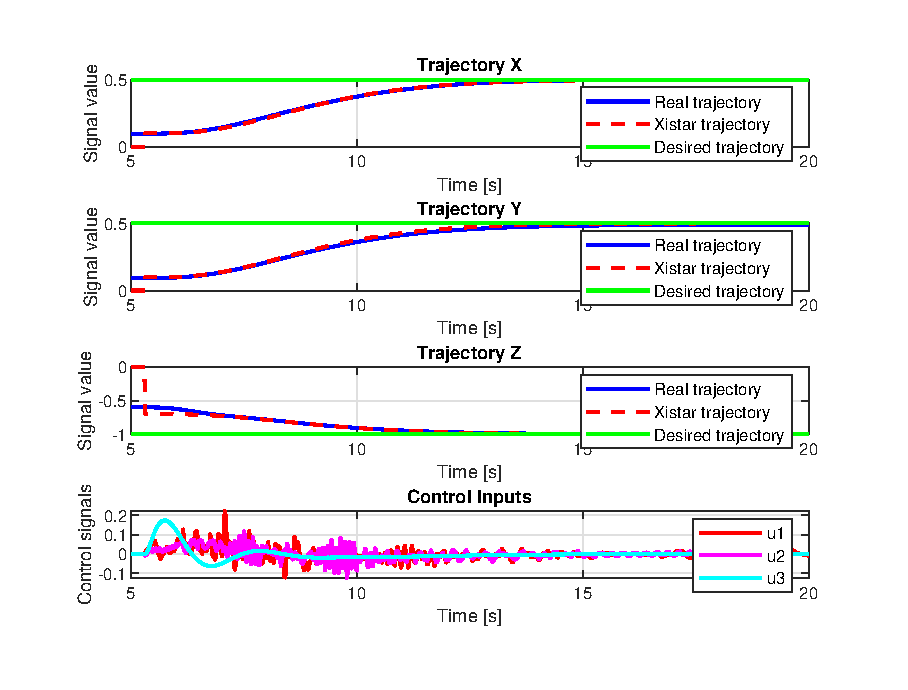
\includegraphics[width=0.8\linewidth]{imgs/section1/noPeaking.eps}
  \caption{Real plant experiment - trajectory tracking without peaking phenomenon.}
  \label{fig:Real_PLant_without_Peaking}
\end{figure}


\begin{figure}[htbp]
  \centering
  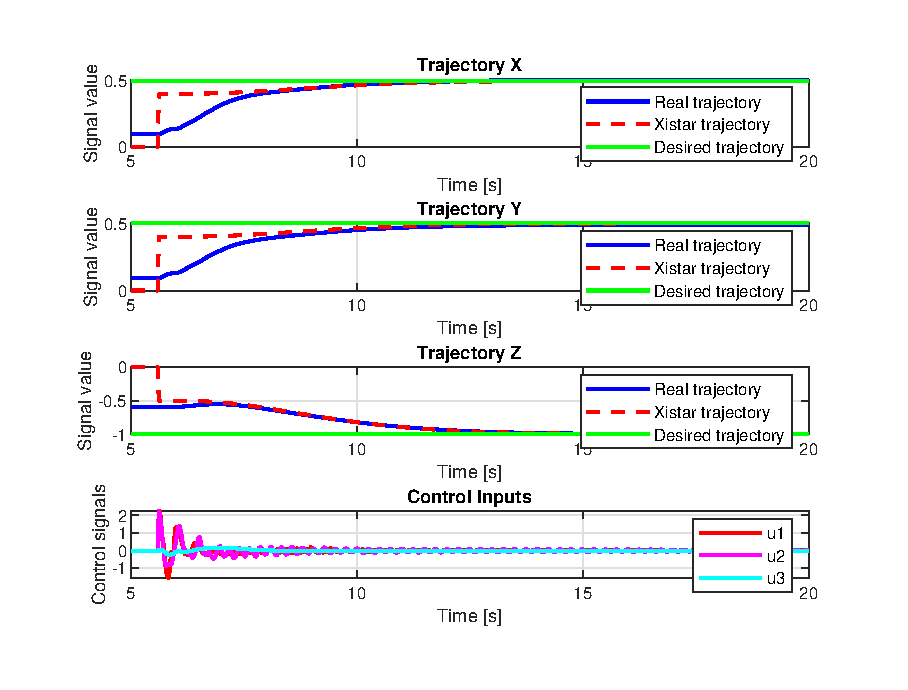
\includegraphics[width=0.8\linewidth]{imgs/section1/midPeaking.eps}
  \caption{Real plant experiment - trajectory tracking with peaking phenomenon.}
  \label{fig:Real_Plant_with_Peaking}
\end{figure}


The set points are reached in both cases with and exponential convergence that 
can be tuned with the time scaling factor \(\epsilon\).


\newpage
\section{Conclusion on the MFC Strategy}
The Model Following Control (MFC) strategy has been presented as a 
robust control technique that ensures a system's output follows a desired 
reference model, even in the presence of uncertainties and disturbances. 
This chapter detailed the theoretical foundations and implementation 
aspects of MFC, emphasizing its two-loop structure: the Model Control 
Loop (MCL) and the Process Control Loop (PCL). The MCL provides nominal 
control based on a theoretical model of the plant, while the PCL compensates 
for perturbations and model uncertainties.

The application of MFC to a crane system demonstrated its effectiveness in 
mitigating the peaking phenomenon, a common issue in high gain control 
strategies. The crane system was modeled with its full nonlinear dynamics, 
and feedback linearization was applied to achieve precise control. The 
simulation results and real plant experiments highlighted the advantages 
of MFC over High Gain control. Specifically, MFC reduced the peaking 
phenomenon and required less input work, making it more suitable for 
real-world applications.

The simpler design of MFC, as proposed by Tietze et al., was also discussed 
and implemented. This design streamlined the control loop dynamics, making 
the control law easier to implement and understand. The simulation and 
experimental results confirmed that the simpler design maintained the 
performance benefits of the original MFC strategy while reducing complexity.

In conclusion, the MFC strategy offers a robust and effective solution 
for systems where precise tracking of a reference trajectory is essential. 
It mitigates the peaking phenomenon, reduces input work, and provides a 
simpler control law compared to traditional high gain control strategies. 
Future work could explore further simplifications of the control architecture 
and the application of MFC to other complex systems.

\newpage

\chapter{Local Stability of high order super-twisting 
         with time and state dependent perturbations}
%\input{Sections/section3}

%======================= CONCLUSION =============================
\chapter*{Conclusion}
\addcontentsline{toc}{chapter}{Conclusion}

\newpage

%récupérer les citation avec "/footnotemark"
\nocite{*}

%choix du style de la biblio
\bibliographystyle{plain}
%inclusion de la biblio
\bibliography{bibliographie.bib}
%voir wiki pour plus d'information sur la syntaxe des entrées d'une bibliographie

%Ne pas numéroter cette partie
\part*{Annexes}
%Rajouter la ligne "Annexes" dans le sommaire
\addcontentsline{toc}{part}{Annexes}

% \input{annexes/panda_structs}

% \input{annexes/nuages_de_points}


\end{document}